

\begin{zkrPlain}{25}\noindent 
	Всхожесть семян данного сорта растений равна $1/7$. Посеяно пять семян. Случайная величина $X$ --- количество невзошедших семян из посеянных. Найдите для этой случайной величины: \par \smallskip\small{ \par \zz ряд распределения (и постройте полигон); \par \zz функцию распределения (и постройте ее график); \par \zz математическое ожидание; \par \zz дисперсию и среднее квадратическое отклонение.\par \par}
 
\end{zkrPlain}

\vfil

\begin{zkrPlain}{25}\noindent 
	Найдите математическое ожидание, дисперсию и вероятность $P(X>a/2)$ непрерывной случайной величины с плотностью вероятностей $f(x)$, заданной графически\footnote{график может быть составлен лишь из участков прямых и парабол.}.\\ \begin{figure}[h!]\centering\small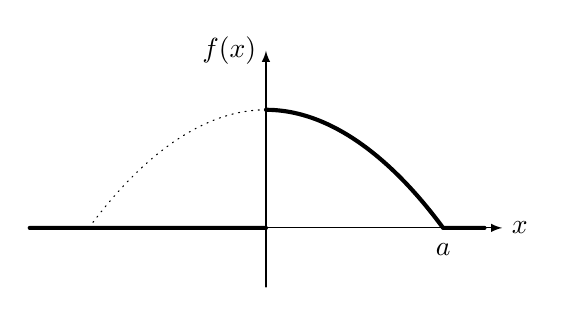
\begin{tikzpicture}[x = 1cm,		y = 1cm,		line join = round,		line cap = round,		> = latex, scale = 1.5,		]\draw[->]	(-2,0) -- (2,0)	node[right]	{$x$};\draw[->]	(0,-.5) --  (0,1.5)	node[left]	{$f(x)$};\draw[line width=1.5pt]	(0,1) parabola (1.5,0) node[below] {$\vphantom{-}a$}			(-2,0) -- (0,0)			(1.5,0) -- (1.85,0);\draw[dotted] (0,1) parabola (-1.5,0);\end{tikzpicture}\end{figure}
 
\end{zkrPlain}

\vfil

\begin{zkrPlain}{25}\noindent 
	Сопротивление партии резисторов распределено по нормальному закону с номинальным средним значением $10$ кОм. Известно, что $84{,}13\%$ резисторов имеют сопротивление меньше $13$ кОм. Найдите: \par \smallskip {\small \par \zz вероятность того, что сопротивление выбранного наудачу резистора окажется в пределах от $9$ кОм до $11$ кОм;\par \zz с надежностью $90\%$ определить максимальное отклонение сопротивления от номинального среднего.}
 
\end{zkrPlain}

\vfil

\begin{zkrPlain}{25}\noindent 
	Вероятность сдачи в срок всех экзаменов студентом университета равна $ 0{,}07 $. Оцените вероятность того, что среди $ 3700 $ студентов число сдавших в срок все экзамены отличается от своего математического ожидания не более чем на $ 44 $. 
 
\end{zkrPlain}

\newpage\setcounter{zad}{0}\setcounter{footnote}{0}



\begin{zkrPlain}{25}\noindent 
	На экзамен пришли пять студентов, уровень подготовки которых примерно одинаков. Вероятность того, что каждый студент завалит экзамен, равна $30\%$ и не зависит от результатов сдачи остальных. Случайная величина $X$ --- число студентов, заваливших экзамен.  Найдите для этой случайной величины: \par \smallskip\small{ \par \zz ряд распределения (и постройте полигон); \par \zz функцию распределения (и постройте ее график); \par \zz математическое ожидание; \par \zz дисперсию и среднее квадратическое отклонение.\par \par}
 
\end{zkrPlain}

\vfil

\begin{zkrPlain}{25}\noindent 
	Найдите математическое ожидание, дисперсию и вероятность $P(X>a/2)$ непрерывной случайной величины с плотностью вероятностей $f(x)$, заданной графически\footnote{график может быть составлен лишь из участков прямых и парабол.}.\\ \begin{figure}[h!]\centering\small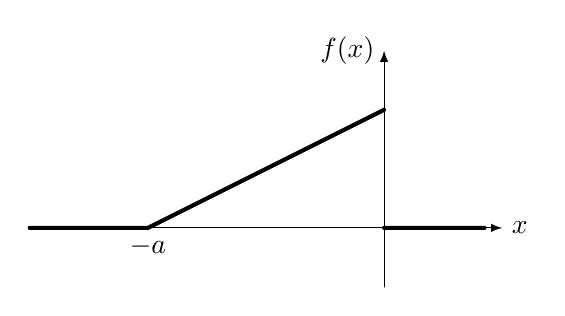
\begin{tikzpicture}[x = 1cm,		y = 1cm,		line join = round,		line cap = round,		> = latex, scale = 1.5,		]\draw[->]	(-3,0) -- (1,0)	node[right]	{$x$};\draw[->]	(0,-.5) --  (0,1.5)	node[left]	{$f(x)$};\draw[line width=1.5pt]		(-2,0) -- (0,1)				(-3,0) -- (-2,0)				(0,0) -- (.85,0);\draw[dotted]		(-2,0) node[below] {$-a$} -- (-2,0);\end{tikzpicture}\end{figure}
 
\end{zkrPlain}

\vfil

\begin{zkrPlain}{25}\noindent 
	Длина переднего рога у африканского белого носорога распределена по нормальному закону с параметром $\sigma = 5$ (см). Всего лишь $2{,}28\%$ белых носорогов имеют рог длиной более $100$ см. Найдите: \par \smallskip {\small \par \zz долю носорогов с рогом длиной от $85$ см до $95$ см;\par \zz квантиль уровня $0{,}3$.}
 
\end{zkrPlain}

\vfil

\begin{zkrPlain}{25}\noindent 
	Электростанция обслуживает сеть на $ 3900 $ электроламп, вероятность включения которых утром равна $ 0{,}6 $. Оцените вероятность того, что число ламп, включенных в сеть сегодня утром, отличается от своего математического ожидания более чем на $ 88 $ (по абсолютной величине). 
 
\end{zkrPlain}

\newpage\setcounter{zad}{0}\setcounter{footnote}{0}



\begin{zkrPlain}{25}\noindent 
	Игральная кость подбрасывается до выпадения шестерки, но не более пяти раз. Случайная величина $X$ --- количество подбрасываний.  Найдите для этой случайной величины: \par \smallskip\small{ \par \zz ряд распределения (и постройте полигон); \par \zz функцию распределения (и постройте ее график); \par \zz математическое ожидание; \par \zz дисперсию и среднее квадратическое отклонение.\par \par}
 
\end{zkrPlain}

\vfil

\begin{zkrPlain}{25}\noindent 
	Найдите математическое ожидание, дисперсию и вероятность $P(X>a/2)$ непрерывной случайной величины с плотностью вероятностей $f(x)$, заданной графически\footnote{график может быть составлен лишь из участков прямых и парабол.}.\\ \begin{figure}[h!]\centering\small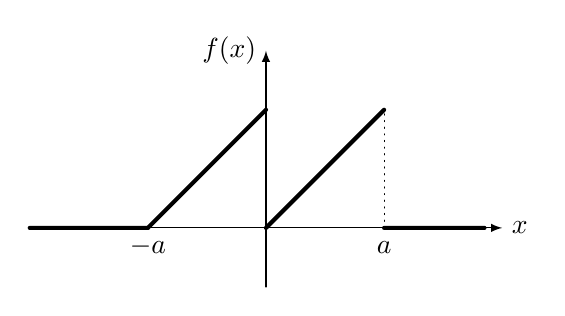
\begin{tikzpicture}[x = 1cm,		y = 1cm,		line join = round,		line cap = round,		> = latex, scale = 1.5,		]\draw[->]	(-2,0) -- (2,0)	node[right]	{$x$};\draw[->]	(0,-.5) --  (0,1.5)	node[left]	{$f(x)$};\draw[line width=1.5pt]		(-1,0) -- (0,1);\draw[line width=1.5pt]		(0,0)  --  (1,1)				(-2,0) -- (-1,0)				(1,0) -- (1.85,0);\draw[dotted]		(-1,0) node[below] {$-a$} -- (-1,0);\draw[dotted]		(1,0)  node[below] {$\vphantom{-}a$} -- (1,1);\end{tikzpicture}\end{figure}
 
\end{zkrPlain}

\vfil

\begin{zkrPlain}{25}\noindent 
	Тесты IQ разрабатываются так, чтобы их результаты описывались нормальным распределением со средним значением $100$ и с таким разбросом, чтобы $25\%$ тестируемых имели IQ ниже $90$. Найдите: \par \smallskip {\small \par \zz вероятность случайному испытуемому получить по результатам теста IQ от $110$  до $120$;\par \zz с помощью правила трех сигм границы, в которых находится IQ большинства людей.}
 
\end{zkrPlain}

\vfil

\begin{zkrPlain}{25}\noindent 
	Среднее значение длины детали $ 14 $ см, а дисперсия --- $ 13 $. Оцените вероятность того, что случайно взятая деталь окажется по длине не менее $ 2 $ и не более $ 26 $ см.
 
\end{zkrPlain}

\newpage\setcounter{zad}{0}\setcounter{footnote}{0}



\begin{zkrPlain}{25}\noindent 
	На маршруте работают три автобуса. Вероятность поломки каждого из них в течение рабочего дня равна $0{,}1$ и не зависит от состояния остальных. Случайная величина $X$ --- число неисправных в течение рабочего дня автобусов.  Найдите для этой случайной величины: \par \smallskip\small{ \par \zz ряд распределения (и постройте полигон); \par \zz функцию распределения (и постройте ее график); \par \zz математическое ожидание; \par \zz дисперсию и среднее квадратическое отклонение.\par \par}
 
\end{zkrPlain}

\vfil

\begin{zkrPlain}{25}\noindent 
	Найдите математическое ожидание, дисперсию и вероятность $P(X>a/2)$ непрерывной случайной величины с плотностью вероятностей $f(x)$, заданной графически\footnote{график может быть составлен лишь из участков прямых и парабол.}.\\ \begin{figure}[h!]\centering\small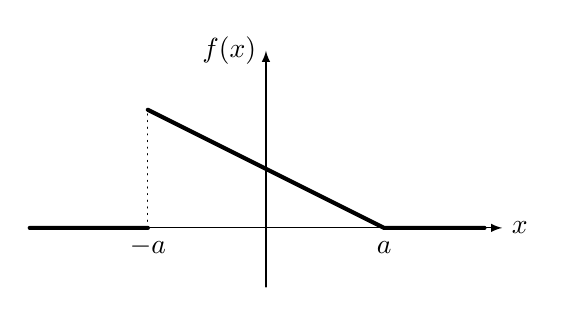
\begin{tikzpicture}[x = 1cm,		y = 1cm,		line join = round,		line cap = round,		> = latex, scale = 1.5,		]\draw[->]	(-2,0) -- (2,0)	node[right]	{$x$};\draw[->]	(0,-.5) --  (0,1.5)	node[left]	{$f(x)$};\draw[line width=1.5pt]		(-1,1) --  (1,0)				(-2,0) -- (-1,0)				(1,0) -- (1.85,0);\draw[dotted]		(-1,0) node[below] {$-a$} -- (-1,1);\draw[dotted]		(1,0)  node[below] {$\vphantom{-}a$} -- (1,0);\end{tikzpicture}\end{figure}
 
\end{zkrPlain}

\vfil

\begin{zkrPlain}{25}\noindent 
	Вес рыб, обитающих в водоеме, подчиняется нормальному закону с параметром $a = 375$ г. Вероятность того, что вес пойманной рыбы меньше $400$ г, равна $0{,}8413$. Найдите: \par \smallskip {\small \par \zz вероятность того, что вес выловленной наудачу рыбы попадет в промежуток от $300$ г до $425$ г;\par \zz квантиль уровня $0{,}7$.}
 
\end{zkrPlain}

\vfil

\begin{zkrPlain}{25}\noindent 
	Вероятность того, что акции, переданные на депозит, будут востребованы, равна $ 0{,}06 $. Оцените вероятность того, что среди $ 2500 $ клиентов от $ 108 $ до $ 192 $ востребуют свои акции.
 
\end{zkrPlain}

\newpage\setcounter{zad}{0}\setcounter{footnote}{0}



\begin{zkrPlain}{25}\noindent 
	Вероятность заболеть гриппом в период эпидемии составляет $3/5$. Рассматривается контрольная группа, состоящая из пяти человек. Случайная величина $X$ --- количество заболевших в период эпидемии человек данной группы.  Найдите для этой случайной величины: \par \smallskip\small{ \par \zz ряд распределения (и постройте полигон); \par \zz функцию распределения (и постройте ее график); \par \zz математическое ожидание; \par \zz дисперсию и среднее квадратическое отклонение.\par \par}
 
\end{zkrPlain}

\vfil

\begin{zkrPlain}{25}\noindent 
	Найдите математическое ожидание, дисперсию и вероятность $P(X>a/2)$ непрерывной случайной величины с плотностью вероятностей $f(x)$, заданной графически\footnote{график может быть составлен лишь из участков прямых и парабол.}.\\ \begin{figure}[h!]\centering\small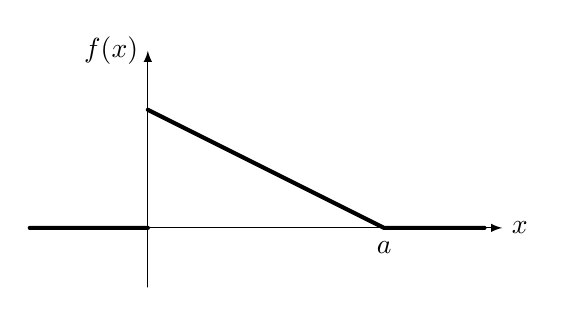
\begin{tikzpicture}[x = 1cm,		y = 1cm,		line join = round,		line cap = round,		> = latex, scale = 1.5,		]\draw[->]	(-1,0) -- (3,0)	node[right]	{$x$};\draw[->]	(0,-.5) --  (0,1.5)	node[left]	{$f(x)$};\draw[line width=1.5pt]		 (0,1) --  (2,0)				(-1,0) -- (0,0)				(2,0) -- (2.85,0);\draw[dotted]		(2,0)  node[below] {$\vphantom{-}a$} -- (2,0);\end{tikzpicture}\end{figure}
 
\end{zkrPlain}

\vfil

\begin{zkrPlain}{25}\noindent 
	Средний рост представителя пигмейских народов гиелли и эфе равен $147$ см. Известно также, что «высоких» людей (выше $1{,}5$ м) среди этих народов — лишь $0{,}13\%$. Учесть, что рост человека (хотя бы и пигмея) распределен нормально. Найдите: \par \smallskip {\small \par \zz долю пигмеев, имеющих рост от $146$ до $148$ см ;\par \zz квантиль уровня $0{,}0227$ описанной случайной величины.}
 
\end{zkrPlain}

\vfil

\begin{zkrPlain}{25}\noindent 
	В среднем $ 5 \% $ работоспособного населения некоторого региона --- безработные. Оцените вероятность того, что уровень безработицы среди обследованных $ 770 $ работоспособных жителей города будет в пределах от $ 3 \% $ до $ 7 \% $.
 
\end{zkrPlain}

\newpage\setcounter{zad}{0}\setcounter{footnote}{0}



\begin{zkrPlain}{25}\noindent 
	Противоположные грани кубика окрашены в красный, зеленый и синий цвета. Кубик подбрасывается 6 раз. Случайная величина $X$ --- количество подбрасываний, в результате которых сверху окажется грань, окрашенная в зеленый цвет.  Найдите для этой случайной величины: \par \smallskip\small{ \par \zz ряд распределения (и постройте полигон); \par \zz функцию распределения (и постройте ее график); \par \zz математическое ожидание; \par \zz дисперсию и среднее квадратическое отклонение.\par \par}
 
\end{zkrPlain}

\vfil

\begin{zkrPlain}{25}\noindent 
	Найдите математическое ожидание, дисперсию и вероятность $P(X>a/2)$ непрерывной случайной величины с плотностью вероятностей $f(x)$, заданной графически\footnote{график может быть составлен лишь из участков прямых и парабол.}.\\ \begin{figure}[h!]\centering\small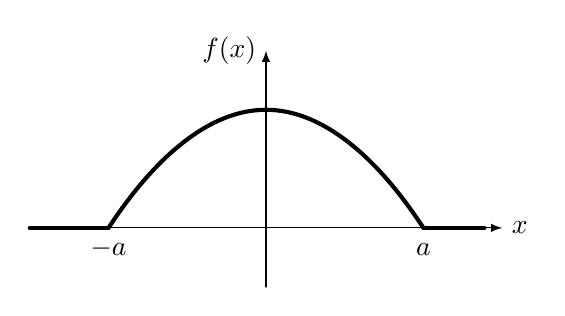
\begin{tikzpicture}[x = 1cm,		y = 1cm,		line join = round,		line cap = round,		> = latex, scale = 1.5,		]\draw[->]	(-2,0) -- (2,0)	node[right]	{$x$};\draw[->]	(0,-.5) --  (0,1.5)	node[left]	{$f(x)$};\draw[line width=1.5pt]		(0,1) parabola (4/3,0) node[below] {$\vphantom{-}a$};\draw[line width=1.5pt]		(0,1) parabola (-4/3,0) node[below] {$-a$};\draw[line width=1.5pt]		(-2,0) -- (-4/3,0)				(4/3,0) -- (1.85,0);\end{tikzpicture}\end{figure}
 
\end{zkrPlain}

\vfil

\begin{zkrPlain}{25}\noindent 
	По статистике ЕГЭ-2012 по математике, $15{,}87\%$ выпускников набрали менее $30$ баллов. Среднее число набранных баллов — $45$. Будем считать число баллов распределенным нормально. Найдите: \par \smallskip {\small \par \zz долю выпускников, набравших более $90$ баллов;\par \zz квантиль уровня $0{,}9522$ числа набранных баллов.}
 
\end{zkrPlain}

\vfil

\begin{zkrPlain}{25}\noindent 
	В течение времени $t$ экслуатируются $ 250 $ приборов. Каждый прибор имеет надежность $ 0{,}8 $ и выходит из строя независимо от других. Оцените вероятность того, что в течение указанного времени выйдут из строя от $ 176 $ до $ 224 $ приборов.
 
\end{zkrPlain}

\newpage\setcounter{zad}{0}\setcounter{footnote}{0}



\begin{zkrPlain}{25}\noindent 
	Экзаменатор задает студенту вопросы до тех пор, пока не получит неверный ответ, но не более 3 вопросов. Вероятность того, что студент верно ответит на первый вопрос, равна $1/8$ и с каждым последующим вопросом увеличивается на $1/8$. Случайная величина $X$ --- число вопросов, заданных студенту.  Найдите для этой случайной величины: \par \smallskip\small{ \par \zz ряд распределения (и постройте полигон); \par \zz функцию распределения (и постройте ее график); \par \zz математическое ожидание; \par \zz дисперсию и среднее квадратическое отклонение.\par \par}
 
\end{zkrPlain}

\vfil

\begin{zkrPlain}{25}\noindent 
	Найдите математическое ожидание, дисперсию и вероятность $P(X>a/2)$ непрерывной случайной величины с плотностью вероятностей $f(x)$, заданной графически\footnote{график может быть составлен лишь из участков прямых и парабол.}.\\ \begin{figure}[h!]\centering\small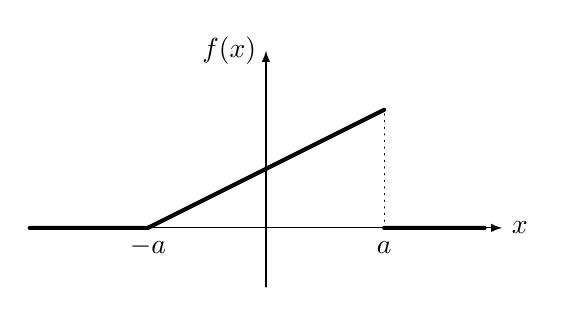
\begin{tikzpicture}[x = 1cm,		y = 1cm,		line join = round,		line cap = round,		> = latex, scale = 1.5,		]\draw[->]	(-2,0) -- (2,0)	node[right]	{$x$};\draw[->]	(0,-.5) --  (0,1.5)	node[left]	{$f(x)$};\draw[line width=1.5pt]		(-1,0) -- (1,1)				(-2,0) -- (-1,0)				(1,0) -- (1.85,0);\draw[dotted]		(-1,0) node[below] {$-a$} -- (-1,0);\draw[dotted]		(1,0)  node[below] {$\vphantom{-}a$} -- (1,1);\end{tikzpicture}\end{figure}
 
\end{zkrPlain}

\vfil

\begin{zkrPlain}{25}\noindent 
	Изменение индекса ценной бумаги на фондовой бирже может быть смоделировано как нормально распределенная случайная величина с параметром $\sigma^2 = 0{,}01$. Известно также, что на следующих торгах с вероятностью $0{,}0228$ изменение индекса будет менее $0{,}8$. Найдите: \par \smallskip {\small \par \zz вероятность того, что на следующих торгах изменение индекса будет больше $1{,}2$.\par \zz нижний квартиль ($x_{0{,}25}$) этой случайной величины.}
 
\end{zkrPlain}

\vfil

\begin{zkrPlain}{25}\noindent 
	Вероятность того, что акции, переданные на депозит, будут востребованы, равна $ 0{,}07 $. Оцените вероятность того, что среди $ 370 $ клиентов от $ 11 $ до $ 41 $ востребуют свои акции.
 
\end{zkrPlain}

\newpage\setcounter{zad}{0}\setcounter{footnote}{0}



\begin{zkrPlain}{25}\noindent 
	Из букв слова СТАТИСТИКА случайным образом выбирают 4 буквы. Случайная величина $X$--- количество гласных букв в выборке. Найдите для этой случайной величины: \par \smallskip\small{ \par \zz ряд распределения (и постройте полигон); \par \zz функцию распределения (и постройте ее график); \par \zz математическое ожидание; \par \zz дисперсию и среднее квадратическое отклонение.\par \par}
 
\end{zkrPlain}

\vfil

\begin{zkrPlain}{25}\noindent 
	Найдите математическое ожидание, дисперсию и вероятность $P(X>a/2)$ непрерывной случайной величины с плотностью вероятностей $f(x)$, заданной графически\footnote{график может быть составлен лишь из участков прямых и парабол.}.\\ \begin{figure}[h!]\centering\small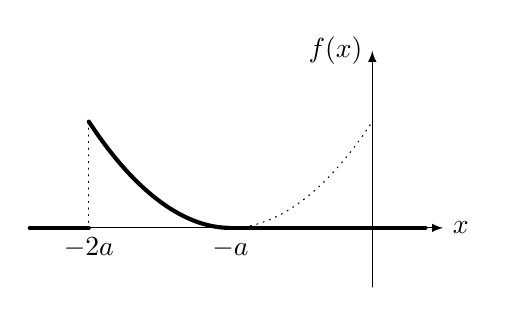
\begin{tikzpicture}[x = 1cm,		y = 1cm,		line join = round,		line cap = round,		> = latex, scale = 1.5,		]\draw[->]	(-.5,0) -- (3,0)	node[right]	{$x$};\draw[->]	(2.4,-.5) --  (2.4,1.5)	node[left]	{$f(x)$};\draw[line width=1.5pt]	(-.5,0) -- (0,0);\draw[line width=1.5pt]	(1.2,0) -- (2.85,0);\draw[dotted]		(1.2,0) parabola (2.4,.9);\draw[line width=1.5pt]		(1.2,0) node[below] {$-a$} parabola (0,.9);\draw[dotted]	(0,.9) -- (0,0) node[below] {$-2a$};\end{tikzpicture}\end{figure}
 
\end{zkrPlain}

\vfil

\begin{zkrPlain}{25}\noindent 
	Коробки с шоколадом упаковываются автоматически. Их средняя масса равна $1{,}2$ кг. Известно, что $9{,}68\%$ коробок имеют массу, меньшую $1{,}07$ кг. Предполагается, что масса коробки распределена нормально. Найдите: \par \smallskip {\small \par \zz процент коробок с массой, превышающей $1140$ г;\par \zz $30\%$-ную точку распределения.}
 
\end{zkrPlain}

\vfil

\begin{zkrPlain}{25}\noindent 
	Среднее значение длины детали $ 30 $ см, а дисперсия --- $ 28 $. Оцените вероятность того, что случайно взятая деталь окажется по длине не менее $ 18 $ и не более $ 42 $ см.
 
\end{zkrPlain}

\newpage\setcounter{zad}{0}\setcounter{footnote}{0}



\begin{zkrPlain}{25}\noindent 
		В рекламных целях торговая фирма вкладывает в каждую десятую единицу товара денежный приз размером 100 рублей. Случайная величина $X$ --- размер выигрыша при трех сделанных покупках.  Найдите для этой случайной величины: \par \smallskip\small{ \par \zz ряд распределения (и постройте полигон); \par \zz функцию распределения (и постройте ее график); \par \zz математическое ожидание; \par \zz дисперсию и среднее квадратическое отклонение.\par \par}
 
\end{zkrPlain}

\vfil

\begin{zkrPlain}{25}\noindent 
	Найдите математическое ожидание, дисперсию и вероятность $P(X>a/2)$ непрерывной случайной величины с плотностью вероятностей $f(x)$, заданной графически\footnote{график может быть составлен лишь из участков прямых и парабол.}.\\ \begin{figure}[h!]\centering\small\begin{tikzpicture}[x = 1cm,		y = 1cm,		line join = round,		line cap = round,		> = latex, scale = 1.5,		]\draw[->]	(-.5,0) -- (3,0)	node[right]	{$x$};\draw[->]	(0,-.5) --  (0,1.5)	node[left]	{$f(x)$};\draw[line width=1.5pt]	(-.5,0) -- (0,0);\draw[line width=1.5pt]	(1.2,0) -- (2.85,0);\draw[dotted]		(1.2,0) parabola (2.4,.9);\draw[line width=1.5pt]		(1.2,0) parabola (0,.9);\draw[dotted]	(1.2,0) -- (1.2,0) node[below]	{$\vphantom{-}a$};\end{tikzpicture}\end{figure}
 
\end{zkrPlain}

\vfil

\begin{zkrPlain}{25}\noindent 
	Уровень воды в реке — случайная величина со средним значением $2{,}5$ м. Вероятность того, что в наудачу выбранный день уровень воды в реке окажется больше $3$ м, равна $0{,}62\%$. Найдите: \par \smallskip {\small \par \zz  вероятность того, что уровень воды в случайный день окажется в пределах от $240$ см до $270$ см;\par \zz $15\%$-ную точку этой случайной величины.}
 
\end{zkrPlain}

\vfil

\begin{zkrPlain}{25}\noindent 
	В среднем $ 7 \% $ работоспособного населения некоторого региона --- безработные. Оцените вероятность того, что уровень безработицы среди обследованных $ 600 $ работоспособных жителей города будет в пределах от $ 4 \% $ до $ 11 \% $.
 
\end{zkrPlain}

\newpage\setcounter{zad}{0}\setcounter{footnote}{0}



\begin{zkrPlain}{25}\noindent 
	Среди 14 монет 8 --- фальшивые. Наудачу вынимают пять монет. Случайная величина $X$ --- количество фальшивых монет в выборке.  Найдите для этой случайной величины: \par \smallskip\small{ \par \zz ряд распределения (и постройте полигон); \par \zz функцию распределения (и постройте ее график); \par \zz математическое ожидание; \par \zz дисперсию и среднее квадратическое отклонение.\par \par}
 
\end{zkrPlain}

\vfil

\begin{zkrPlain}{25}\noindent 
	Найдите математическое ожидание, дисперсию и вероятность $P(X>a/2)$ непрерывной случайной величины с плотностью вероятностей $f(x)$, заданной графически\footnote{график может быть составлен лишь из участков прямых и парабол.}.\\ \begin{figure}[h!]\centering\small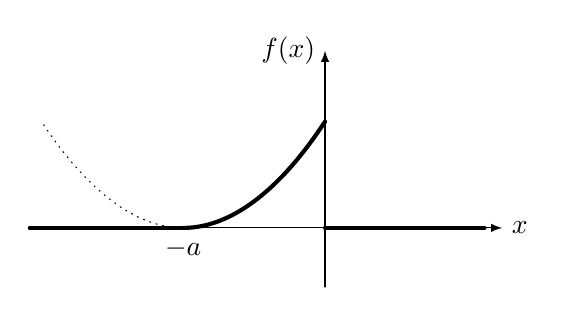
\begin{tikzpicture}[x = 1cm,		y = 1cm,		line join = round,		line cap = round,		> = latex, scale = 1.5,		]\draw[->]	(-2.5,0) -- (1.5,0)	node[right]	{$x$};\draw[->]	(0,-.5) --  (0,1.5)	node[left]	{$f(x)$};\draw[line width=1.5pt]		(-1.2,0) node[below] {$-a$} parabola (0,.9);\draw[line width=1.5pt]		(-2.5,0) -- (-1.2,0)				(0,0) -- (1.35,0);\draw[dotted]	(-1.2,0) parabola (-2.4,.9);\end{tikzpicture}\end{figure}
 
\end{zkrPlain}

\vfil

\begin{zkrPlain}{25}\noindent 
	Вес гигантского броненосца — нормально распределенная случайная величина. Известно, что $74{,}75\%$ этих животных в весе не превышают $27$ кг, а тяжелее $30$ кг — лишь $4{,}78\%$ броненосцев. Найдите: \par \smallskip {\small \par \zz вероятность случайно встретить в джунглях броненосца весом менее $22$ кг;\par \zz $9{,}12\%$-ную точку данной случайной величины.}
 
\end{zkrPlain}

\vfil

\begin{zkrPlain}{25}\noindent 
	Вероятность сдачи в срок всех экзаменов студентом университета равна $ 0{,}08 $. Оцените вероятность того, что среди $ 530 $ студентов число сдавших в срок все экзамены отличается от своего математического ожидания не более чем на $ 24 $. 
 
\end{zkrPlain}

\newpage\setcounter{zad}{0}\setcounter{footnote}{0}



\begin{zkrPlain}{25}\noindent 
	В кошельке 4 двухрублевые и 3 пятирублевые монеты. Наудачу извлекают пять монет. Случайная величина $X$ --- сумма денег в рублях, которую составляют извлеченные монеты.  Найдите для этой случайной величины: \par \smallskip\small{ \par \zz ряд распределения (и постройте полигон); \par \zz функцию распределения (и постройте ее график); \par \zz математическое ожидание; \par \zz дисперсию и среднее квадратическое отклонение.\par \par}
 
\end{zkrPlain}

\vfil

\begin{zkrPlain}{25}\noindent 
	Найдите математическое ожидание, дисперсию и вероятность $P(X>a/2)$ непрерывной случайной величины с плотностью вероятностей $f(x)$, заданной графически\footnote{график может быть составлен лишь из участков прямых и парабол.}.\\ \begin{figure}[h!]\centering\small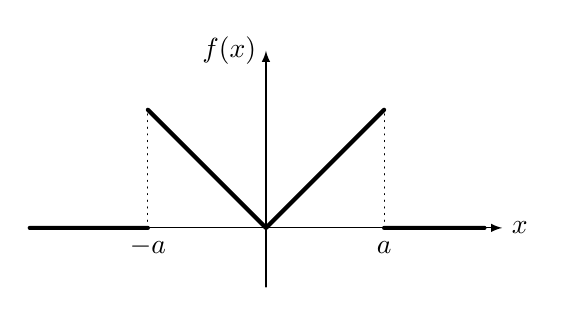
\begin{tikzpicture}[x = 1cm,		y = 1cm,		line join = round,		line cap = round,		> = latex, scale = 1.5,		]\draw[->]	(-2,0) -- (2,0)	node[right]	{$x$};\draw[->]	(0,-.5) --  (0,1.5)	node[left]	{$f(x)$};\draw[line width=1.5pt]		(-1,1) -- (0,0) --  (1,1)				(-2,0) -- (-1,0)				(1,0) -- (1.85,0);\draw[dotted]		(-1,0) node[below] {$-a$} -- (-1,1);\draw[dotted]		(1,0)  node[below] {$\vphantom{-}a$} -- (1,1);\end{tikzpicture}\end{figure}
 
\end{zkrPlain}

\vfil

\begin{zkrPlain}{25}\noindent 
	Вес товаров, помещаемых в контейнер определенного размера, — нормально распределенная случайная величина. Известно, что $34{,}46\%$ контейнеров имеют чистый вес меньше $8$ тонн и $21{,}19\%$ имеют вес больше, чем $14$ тонн. Найдите: \par \smallskip {\small \par \zz средний вес одного контейнера; \par \zz с надежностью $0{,}9$ максимальное отклонение веса контейнера от среднего значения. }
 
\end{zkrPlain}

\vfil

\begin{zkrPlain}{25}\noindent 
	В течение времени $t$ экслуатируются $ 560 $ приборов. Каждый прибор имеет надежность $ 0{,}5 $ и выходит из строя независимо от других. Оцените вероятность того, что в течение указанного времени выйдут из строя от $ 242 $ до $ 318 $ приборов.
 
\end{zkrPlain}

\newpage\setcounter{zad}{0}\setcounter{footnote}{0}



\begin{zkrPlain}{25}\noindent 
	В ящике находятся 14 деталей, среди которых 6 бракованные. Наудачу из этих деталей вынимаются 4. Случайная величина $X$ --- количество бракованных деталей в выборке.  Найдите для этой случайной величины: \par \smallskip\small{ \par \zz ряд распределения (и постройте полигон); \par \zz функцию распределения (и постройте ее график); \par \zz математическое ожидание; \par \zz дисперсию и среднее квадратическое отклонение.\par \par}
 
\end{zkrPlain}

\vfil

\begin{zkrPlain}{25}\noindent 
	Найдите математическое ожидание, дисперсию и вероятность $P(X>a/2)$ непрерывной случайной величины с плотностью вероятностей $f(x)$, заданной графически\footnote{график может быть составлен лишь из участков прямых и парабол.}.\\ \begin{figure}[h!]\centering\small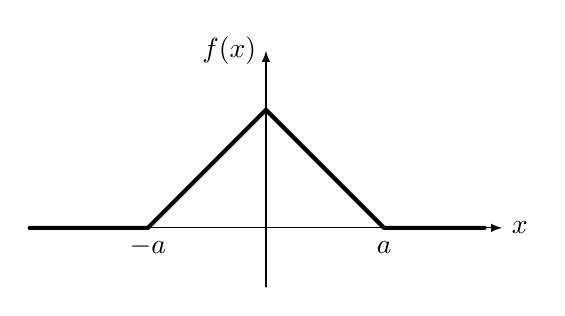
\begin{tikzpicture}[x = 1cm,		y = 1cm,		line join = round,		line cap = round,		> = latex, scale = 1.5,		]\draw[->]	(-2,0) -- (2,0)	node[right]	{$x$};\draw[->]	(0,-.5) --  (0,1.5)	node[left]	{$f(x)$};\draw[line width=1.5pt]		(-1,0) -- (0,1) --  (1,0)				(-2,0) -- (-1,0)				(1,0) -- (1.85,0);\draw[dotted]		(-1,0) node[below] {$-a$} -- (-1,0);\draw[dotted]		(1,0)  node[below] {$\vphantom{-}a$} -- (1,0);\end{tikzpicture}\end{figure}
 
\end{zkrPlain}

\vfil

\begin{zkrPlain}{25}\noindent 
	Прочность пряжи приблизительно следует нормальному закону распределения. Средняя прочность пряжи — $245$ сн\footnote{1 сн (стен [тэ]) = 1000 ньютонов}. $1{,}22\%$ пряжи имеет прочность менее $200$ сн. Найдите: \par \smallskip {\small \par \zz вероятность того, что прочность окажется в интервале от $220$ сн до $270$ сн.\par \zz оценить наиболее вероятные границы прочности с помощью правила трех сигм.}
 
\end{zkrPlain}

\vfil

\begin{zkrPlain}{25}\noindent 
	Электростанция обслуживает сеть на $ 6100 $ электроламп, вероятность включения которых утром равна $ 0{,}8 $. Оцените вероятность того, что число ламп, включенных в сеть сегодня утром, отличается от своего математического ожидания более чем на $ 64 $ (по абсолютной величине). 
 
\end{zkrPlain}

\newpage\setcounter{zad}{0}\setcounter{footnote}{0}



\begin{zkrPlain}{25}\noindent 
	Стрелок ведет стрельбу по цели с вероятностью промаха при каждом выстреле $45\%$. За каждое попадание он получает 10 очков, а в случае промаха очков ему не начисляют. Случайная величина $X$ --- число очков, полученных стрелком за 4 выстрелов.  Найдите для этой случайной величины: \par \smallskip\small{ \par \zz ряд распределения (и постройте полигон); \par \zz функцию распределения (и постройте ее график); \par \zz математическое ожидание; \par \zz дисперсию и среднее квадратическое отклонение.\par \par}
 
\end{zkrPlain}

\vfil

\begin{zkrPlain}{25}\noindent 
	Найдите математическое ожидание, дисперсию и вероятность $P(X>a/2)$ непрерывной случайной величины с плотностью вероятностей $f(x)$, заданной графически\footnote{график может быть составлен лишь из участков прямых и парабол.}.\\ \begin{figure}[h!]\centering\small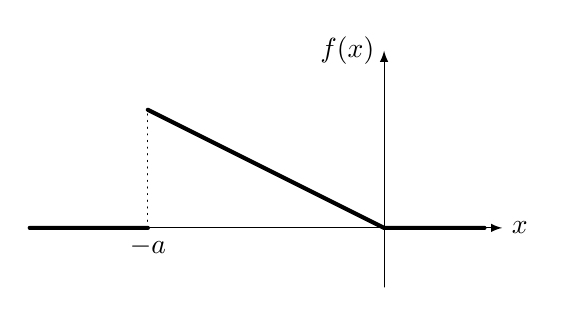
\begin{tikzpicture}[x = 1cm,		y = 1cm,		line join = round,		line cap = round,		> = latex, scale = 1.5,		]\draw[->]	(-3,0) -- (1,0)	node[right]	{$x$};\draw[->]	(0,-.5) --  (0,1.5)	node[left]	{$f(x)$};\draw[line width=1.5pt]		(-2,1) -- (0,0)				(-3,0) -- (-2,0)				(0,0) -- (.85,0);\draw[dotted]		(-2,0) node[below] {$-a$} -- (-2,1);\end{tikzpicture}\end{figure}
 
\end{zkrPlain}

\vfil

\begin{zkrPlain}{25}\noindent 
	Словарный запас английского языка у изучающих его — случайная величина, распределенная нормально. Известно, что в среднем этот запас составляет 8000 слов. Кроме этого, имеются данные, согласно которым $30{,}85\%$ изучающих имеют словарный запас менее $6000$ слов. Найдите: \par \smallskip {\small \par \zz долю изучающих английский со словарным запасом более $15000$ слов;\par \zz нижний квартиль ($x_{0{,}25}$)указанной случайной величины.}
 
\end{zkrPlain}

\vfil

\begin{zkrPlain}{25}\noindent 
	Среднее значение длины детали $ 275 $ см, а дисперсия --- $ 261 $. Оцените вероятность того, что случайно взятая деталь окажется по длине не менее $ 253 $ и не более $ 297 $ см.
 
\end{zkrPlain}

\newpage\setcounter{zad}{0}\setcounter{footnote}{0}



\begin{zkrPlain}{25}\noindent 
	В корзине 7 синих и 5 красных мячей. Наудачу вынимают четыре мяча. Случайная величина $X$ --- количество красных мячей в выборке.  Найдите для этой случайной величины: \par \smallskip\small{ \par \zz ряд распределения (и постройте полигон); \par \zz функцию распределения (и постройте ее график); \par \zz математическое ожидание; \par \zz дисперсию и среднее квадратическое отклонение.\par \par}
 
\end{zkrPlain}

\vfil

\begin{zkrPlain}{25}\noindent 
	Найдите математическое ожидание, дисперсию и вероятность $P(X>a/2)$ непрерывной случайной величины с плотностью вероятностей $f(x)$, заданной графически\footnote{график может быть составлен лишь из участков прямых и парабол.}.\\ \begin{figure}[h!]\centering\small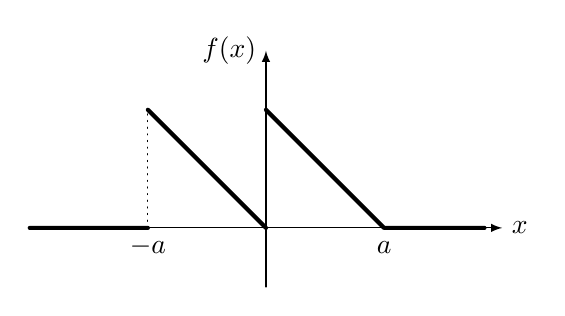
\begin{tikzpicture}[x = 1cm,		y = 1cm,		line join = round,		line cap = round,		> = latex, scale = 1.5,		]\draw[->]	(-2,0) -- (2,0)	node[right]	{$x$};\draw[->]	(0,-.5) --  (0,1.5)	node[left]	{$f(x)$};\draw[line width=1.5pt]		(-1,1) -- (0,0);\draw[line width=1.5pt]		(0,1) --  (1,0)				(-2,0) -- (-1,0)				(1,0) -- (1.85,0);\draw[dotted]		(-1,0) node[below] {$-a$} -- (-1,1);\draw[dotted]		(1,0)  node[below] {$\vphantom{-}a$} -- (1,0);\end{tikzpicture}\end{figure}
 
\end{zkrPlain}

\vfil

\begin{zkrPlain}{25}\noindent 
	Отклонение количества изюма в кексах от среднего больше $15$ изюмин на кекс встречается в $68{,}27\%$ кексов. Кроме этого, замечено, что в $25{,}25\%$ случаев число изюминок в кексе меньше $70$. Найдите: \par \smallskip {\small \par \zz вероятность того, что изюминок в купленном кексе окажется от $90$ до $100$;\par \zz $4{,}78\%$-ную точку числа изюмин.}
 
\end{zkrPlain}

\vfil

\begin{zkrPlain}{25}\noindent 
	Вероятность сдачи в срок всех экзаменов студентом университета равна $ 0{,}06 $. Оцените вероятность того, что среди $ 630 $ студентов число сдавших в срок все экзамены отличается от своего математического ожидания не более чем на $ 24 $. 
 
\end{zkrPlain}

\newpage\setcounter{zad}{0}\setcounter{footnote}{0}



\begin{zkrPlain}{25}\noindent 
	Среди партии шарфов, поступивших в магазин, $70 \%$ составляют однотонные шарфы, а остальные --- пестрые. Покупатель из этих шарфов случайным образом выбирает три. Случайная величина $X$ --- количество пестрых шарфов в выборке.  Найдите для этой случайной величины: \par \smallskip\small{ \par \zz ряд распределения (и постройте полигон); \par \zz функцию распределения (и постройте ее график); \par \zz математическое ожидание; \par \zz дисперсию и среднее квадратическое отклонение.\par \par}
 
\end{zkrPlain}

\vfil

\begin{zkrPlain}{25}\noindent 
	Найдите математическое ожидание, дисперсию и вероятность $P(X>a/2)$ непрерывной случайной величины с плотностью вероятностей $f(x)$, заданной графически\footnote{график может быть составлен лишь из участков прямых и парабол.}.\\ \begin{figure}[h!]\centering\small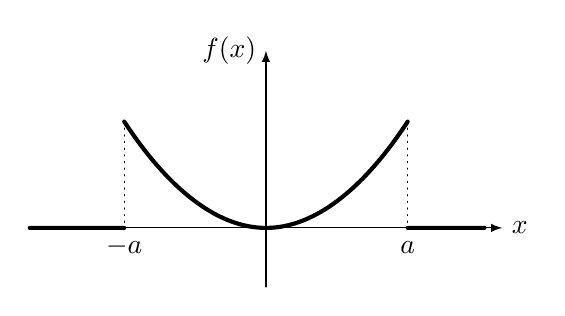
\begin{tikzpicture}[x = 1cm,		y = 1cm,		line join = round,		line cap = round,		> = latex, scale = 1.5,		]\draw[->]	(-2,0) -- (2,0)	node[right]	{$x$};\draw[->]	(0,-.5) --  (0,1.5)	node[left]	{$f(x)$};\draw[line width=1.5pt]		(0,0) parabola (1.2,.9);\draw[line width=1.5pt]		(0,0) parabola (-1.2,.9)				(-2,0) -- (-1.2,0)				(1.2,0) -- (1.85,0);\draw[dotted]	(-1.2,.9) -- (-1.2,0) node[below]	{$-a$};\draw[dotted]	(1.2,.9) -- (1.2,0) node[below]	{$\vphantom{-}a$};\end{tikzpicture}\end{figure}
 
\end{zkrPlain}

\vfil

\begin{zkrPlain}{25}\noindent 
	По статистике ЕГЭ-2012 (русский язык), $7{,}66\%$ выпускников набрали менее $40$ баллов. Известно также, что $23{,}75\%$ выпускников получили более $70$ баллов. Считаем распределение баллов нормальным. Найдите: \par \smallskip {\small \par \zz средний балл по русскому языку;\par \zz долю отличников, получивших более $90$ баллов.}
 
\end{zkrPlain}

\vfil

\begin{zkrPlain}{25}\noindent 
	В течение времени $t$ экслуатируются $ 2000 $ приборов. Каждый прибор имеет надежность $ 0{,}6 $ и выходит из строя независимо от других. Оцените вероятность того, что в течение указанного времени выйдут из строя от $ 1130 $ до $ 1270 $ приборов.
 
\end{zkrPlain}

\newpage\setcounter{zad}{0}\setcounter{footnote}{0}



\begin{zkrPlain}{25}\noindent 
	В контрольной работе шесть задач. Вероятность правильного решения студентом каждой задачи равна $25\%$ и не зависит от правильности решения остальных. Случайная величина $X$ --- количество правильно решенных задач.  Найдите для этой случайной величины: \par \smallskip\small{ \par \zz ряд распределения (и постройте полигон); \par \zz функцию распределения (и постройте ее график); \par \zz математическое ожидание; \par \zz дисперсию и среднее квадратическое отклонение.\par \par}
 
\end{zkrPlain}

\vfil

\begin{zkrPlain}{25}\noindent 
	Найдите математическое ожидание, дисперсию и вероятность $P(X>a/2)$ непрерывной случайной величины с плотностью вероятностей $f(x)$, заданной графически\footnote{график может быть составлен лишь из участков прямых и парабол.}.\\ \begin{figure}[h!]\centering\small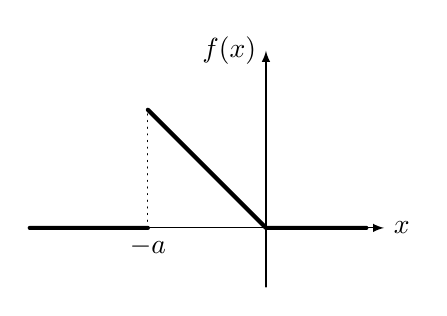
\begin{tikzpicture}[x = 1cm,		y = 1cm,		line join = round,		line cap = round,		> = latex, scale = 1.5,		]\draw[->]	(-2,0) -- (1,0)	node[right]	{$x$};\draw[->]	(0,-.5) --  (0,1.5)	node[left]	{$f(x)$};\draw[line width=1.5pt]		(-1,1) -- (0,0)				(-2,0) -- (-1,0)				(0,0) -- (.85,0);\draw[dotted]		(-1,0) node[below] {$-a$} -- (-1,1);\end{tikzpicture}\end{figure}
 
\end{zkrPlain}

\vfil

\begin{zkrPlain}{25}\noindent 
	Средний вес расфасованных пакетов со стиральным порошком $930$ г, но, как правило, около $6{,}68\%$ пакетов тяжелее $960$ г. Считаем, что вес пакетов распределен нормально. Найдите: \par \smallskip {\small \par \zz долю пакетов, имеющих вес до $900$ г.\par \zz Требуется, чтобы не более $4\%$ пакетов содержали меньше $900$ г порошка. На какой средний вес пакетов нужно переналадить фасовочный автомат для выполнения этого задания?}
 
\end{zkrPlain}

\vfil

\begin{zkrPlain}{25}\noindent 
	Электростанция обслуживает сеть на $ 7100 $ электроламп, вероятность включения которых утром равна $ 0{,}7 $. Оцените вероятность того, что число ламп, включенных в сеть сегодня утром, отличается от своего математического ожидания более чем на $ 53 $ (по абсолютной величине). 
 
\end{zkrPlain}

\newpage\setcounter{zad}{0}\setcounter{footnote}{0}



\begin{zkrPlain}{25}\noindent 
	Сотрудник лаборатории проводит пять независимых опытов. Вероятность успешного опыта равна $25\%$ и не зависит от успешности предыдущих опытов. Случайная величина $X$ --- число неудачных опытов.  Найдите для этой случайной величины: \par \smallskip\small{ \par \zz ряд распределения (и постройте полигон); \par \zz функцию распределения (и постройте ее график); \par \zz математическое ожидание; \par \zz дисперсию и среднее квадратическое отклонение.\par \par}
 
\end{zkrPlain}

\vfil

\begin{zkrPlain}{25}\noindent 
	Найдите математическое ожидание, дисперсию и вероятность $P(X>a/2)$ непрерывной случайной величины с плотностью вероятностей $f(x)$, заданной графически\footnote{график может быть составлен лишь из участков прямых и парабол.}.\\ \begin{figure}[h!]\centering\small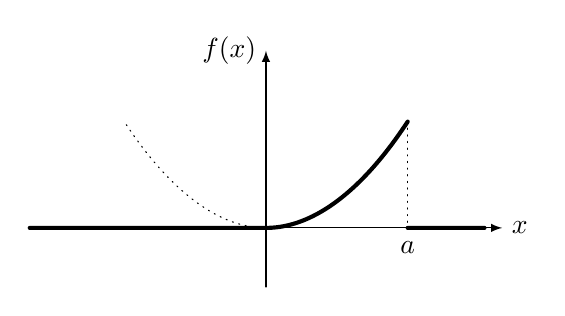
\begin{tikzpicture}[x = 1cm,		y = 1cm,		line join = round,		line cap = round,		> = latex, scale = 1.5,				]\draw[->]	(-2,0) -- (2,0)	node[right]	{$x$};\draw[->]	(0,-.5) --  (0,1.5)	node[left]	{$f(x)$};\draw[line width=1.5pt]	(0,0) parabola (1.2,.9)			(-2,0) -- (0,0)			(1.2,0) -- (1.85,0);\draw[dotted]	(0,0) parabola (-1.2,.9);\draw[dotted]	(1.2,.9) -- (1.2,0)	node[below]{$\vphantom{-}a$};\end{tikzpicture}\end{figure}
 
\end{zkrPlain}

\vfil

\begin{zkrPlain}{25}\noindent 
	Средняя высота секвойи вечнозеленой  — порядка {$90$~м}. Примерно $1{,}31\%$ этих деревьев достигают в высоту $110$~м и более. Будем считать, что высота секвойи — нормально распределенная случайная величина. Найдите: \par \smallskip {\small \par \zz вероятность обнаружить секвойю высотой от $95$ до $105$ м;\par \zz вероятность того, что отклонение высоты случайной секвойи от средней составит не более десяти метров (по абсолютной величине).}
 
\end{zkrPlain}

\vfil

\begin{zkrPlain}{25}\noindent 
	В среднем $ 6 \% $ работоспособного населения некоторого региона --- безработные. Оцените вероятность того, что уровень безработицы среди обследованных $ 650 $ работоспособных жителей города будет в пределах от $ 4 \% $ до $ 8 \% $.
 
\end{zkrPlain}

\newpage\setcounter{zad}{0}\setcounter{footnote}{0}



\begin{zkrPlain}{25}\noindent 
	Экзаменатор задает студенту вопросы до тех пор, пока не получит верный ответ, но не более 3 вопросов. Вероятность того, что студент неверно ответит на первый вопрос, равна $6/7$ и с каждым последующим вопросом уменьшается на $1/7$. Случайная величина $X$ --- число вопросов, заданных студенту.  Найдите для этой случайной величины: \par \smallskip\small{ \par \zz ряд распределения (и постройте полигон); \par \zz функцию распределения (и постройте ее график); \par \zz математическое ожидание; \par \zz дисперсию и среднее квадратическое отклонение.\par \par}
 
\end{zkrPlain}

\vfil

\begin{zkrPlain}{25}\noindent 
	Найдите математическое ожидание, дисперсию и вероятность $P(X>a/2)$ непрерывной случайной величины с плотностью вероятностей $f(x)$, заданной графически\footnote{график может быть составлен лишь из участков прямых и парабол.}.\\ \begin{figure}[h!]\centering\small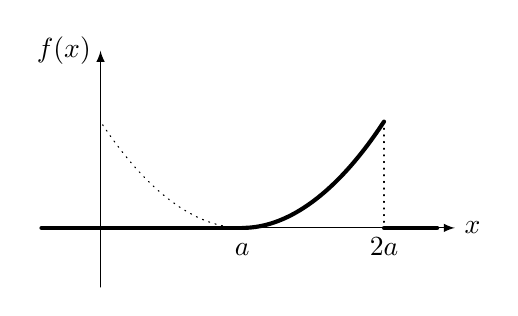
\begin{tikzpicture}[x = 1cm,		y = 1cm,		line join = round,		line cap = round,		> = latex, scale = 1.5,		]\draw[->]	(-.5,0) -- (3,0)	node[right]	{$x$};\draw[->]	(0,-.5) --  (0,1.5)	node[left]	{$f(x)$};\draw[line width=1.5pt]	(-.5,0) -- (1.2,0);\draw[line width=1.5pt]	(2.4,0) -- (2.85,0);\draw[line width=1.5pt]		(1.2,0) node[below] {$\vphantom{-}a$} parabola (2.4,.9);\draw[dotted]		(1.2,0) parabola (0,.9);\draw[dotted]	(2.4,.9) -- (2.4,0)  node[below] {$\vphantom{-}2a$};\end{tikzpicture}\end{figure}
 
\end{zkrPlain}

\vfil

\begin{zkrPlain}{25}\noindent 
	Считаем, что рост императорского пингвина распределен нормально со средним квадратическим отклонением в три сантиметра. Известно, что $15{,}87\%$ императорских пингвинов имеют рост ниже $112$ см. Найдите: \par \smallskip {\small \par \zz долю императорских пингвинов с ростом от $116$ до $122$ см.;\par \zz с надежностью $0{,}9$ определить максимальное отклонение роста пингвина от его среднего значения.}
 
\end{zkrPlain}

\vfil

\begin{zkrPlain}{25}\noindent 
	Вероятность того, что акции, переданные на депозит, будут востребованы, равна $ 0{,}07 $. Оцените вероятность того, что среди $ 590 $ клиентов от $ 21 $ до $ 61 $ востребуют свои акции.
 
\end{zkrPlain}

\newpage\setcounter{zad}{0}\setcounter{footnote}{0}



\begin{zkrPlain}{25}\noindent 
	Секретариат фирмы оборудован четырьмя независимо работающими компьютерами. Вероятность отказа каждого из них в течение рабочего дня равна $0{,}1$. Случайная величина $X$ --- количество отказавших в течение рабочего дня компьютеров.  Найдите для этой случайной величины: \par \smallskip\small{ \par \zz ряд распределения (и постройте полигон); \par \zz функцию распределения (и постройте ее график); \par \zz математическое ожидание; \par \zz дисперсию и среднее квадратическое отклонение.\par \par}
 
\end{zkrPlain}

\vfil

\begin{zkrPlain}{25}\noindent 
	Найдите математическое ожидание, дисперсию и вероятность $P(X>a/2)$ непрерывной случайной величины с плотностью вероятностей $f(x)$, заданной графически\footnote{график может быть составлен лишь из участков прямых и парабол.}.\\ \begin{figure}[h!]\centering\small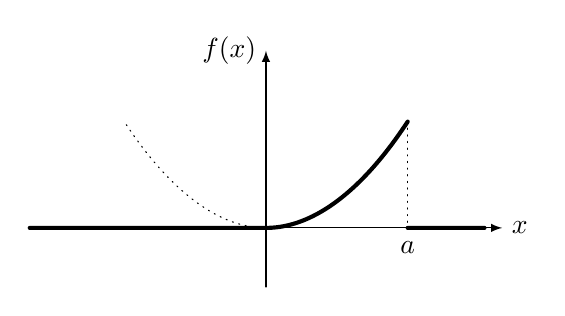
\begin{tikzpicture}[x = 1cm,		y = 1cm,		line join = round,		line cap = round,		> = latex, scale = 1.5,				]\draw[->]	(-2,0) -- (2,0)	node[right]	{$x$};\draw[->]	(0,-.5) --  (0,1.5)	node[left]	{$f(x)$};\draw[line width=1.5pt]	(0,0) parabola (1.2,.9)			(-2,0) -- (0,0)			(1.2,0) -- (1.85,0);\draw[dotted]	(0,0) parabola (-1.2,.9);\draw[dotted]	(1.2,.9) -- (1.2,0)	node[below]{$\vphantom{-}a$};\end{tikzpicture}\end{figure}
 
\end{zkrPlain}

\vfil

\begin{zkrPlain}{25}\noindent 
	Максимальная урожайность большей части современных сортов картофеля — нормально распределенная случайная величина, принимающая $99{,}73\%$ своих значений в интервале $420-780$ ц/га. Найдите: \par \smallskip {\small \par \zz вероятность того, что урожайность высаженного картофеля в данном году составит от $650$ до $700$ ц/га;\par \zz $36{,}94\%$-ную точку указанной случайной величины.}
 
\end{zkrPlain}

\vfil

\begin{zkrPlain}{25}\noindent 
	В среднем $ 6 \% $ работоспособного населения некоторого региона --- безработные. Оцените вероятность того, что уровень безработицы среди обследованных $ 740 $ работоспособных жителей города будет в пределах от $ 4 \% $ до $ 7 \% $.
 
\end{zkrPlain}

\newpage\setcounter{zad}{0}\setcounter{footnote}{0}



\begin{zkrPlain}{25}\noindent 
	В ящике находятся 5 белых и 5 черных шаров. Случайным образом последовательно вынимаются шары до появления белого шара. Шары не возвращаются в ящик. Случайная величина $X$ --- количество вынутых шаров.  Найдите для этой случайной величины: \par \smallskip\small{ \par \zz ряд распределения (и постройте полигон); \par \zz функцию распределения (и постройте ее график); \par \zz математическое ожидание; \par \zz дисперсию и среднее квадратическое отклонение.\par \par}
 
\end{zkrPlain}

\vfil

\begin{zkrPlain}{25}\noindent 
	Найдите математическое ожидание, дисперсию и вероятность $P(X>a/2)$ непрерывной случайной величины с плотностью вероятностей $f(x)$, заданной графически\footnote{график может быть составлен лишь из участков прямых и парабол.}.\\ \begin{figure}[h!]\centering\small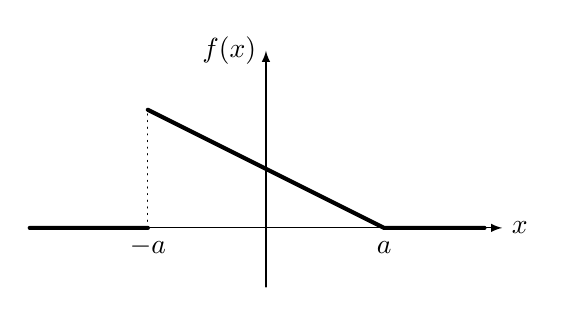
\begin{tikzpicture}[x = 1cm,		y = 1cm,		line join = round,		line cap = round,		> = latex, scale = 1.5,		]\draw[->]	(-2,0) -- (2,0)	node[right]	{$x$};\draw[->]	(0,-.5) --  (0,1.5)	node[left]	{$f(x)$};\draw[line width=1.5pt]		(-1,1) --  (1,0)				(-2,0) -- (-1,0)				(1,0) -- (1.85,0);\draw[dotted]		(-1,0) node[below] {$-a$} -- (-1,1);\draw[dotted]		(1,0)  node[below] {$\vphantom{-}a$} -- (1,0);\end{tikzpicture}\end{figure}
 
\end{zkrPlain}

\vfil

\begin{zkrPlain}{25}\noindent 
	Спортсмен бросает копье. Дальность полета — нормально распределенная величина со средним значением $70$ м. По статистике $2{,}28\%$ бросков, как правило, оказываются неудачными (дальность полета менее $60$ м).  Найдите: \par \smallskip {\small \par \zz  вероятность того, что копье упадет на расстоянии от $65$ м до $75$ м.\par \zz нижний квартиль распределения ($x_{0{,}25}$).}
 
\end{zkrPlain}

\vfil

\begin{zkrPlain}{25}\noindent 
	Электростанция обслуживает сеть на $ 7700 $ электроламп, вероятность включения которых утром равна $ 0{,}5 $. Оцените вероятность того, что число ламп, включенных в сеть сегодня утром, отличается от своего математического ожидания более чем на $ 89 $ (по абсолютной величине). 
 
\end{zkrPlain}

\newpage\setcounter{zad}{0}\setcounter{footnote}{0}



\begin{zkrPlain}{25}\noindent 
	В рекламных целях торговая фирма вкладывает в каждую десятую единицу товара денежный приз размером 100 рублей. Случайная величина $X$ --- размер выигрыша при трех сделанных покупках.  Найдите для этой случайной величины: \par \smallskip\small{ \par \zz ряд распределения (и постройте полигон); \par \zz функцию распределения (и постройте ее график); \par \zz математическое ожидание; \par \zz дисперсию и среднее квадратическое отклонение.\par \par}
 
\end{zkrPlain}

\vfil

\begin{zkrPlain}{25}\noindent 
	Найдите математическое ожидание, дисперсию и вероятность $P(X>a/2)$ непрерывной случайной величины с плотностью вероятностей $f(x)$, заданной графически\footnote{график может быть составлен лишь из участков прямых и парабол.}.\\ \begin{figure}[h!]\centering\small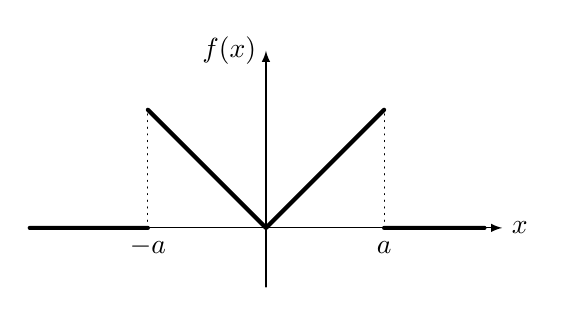
\begin{tikzpicture}[x = 1cm,		y = 1cm,		line join = round,		line cap = round,		> = latex, scale = 1.5,		]\draw[->]	(-2,0) -- (2,0)	node[right]	{$x$};\draw[->]	(0,-.5) --  (0,1.5)	node[left]	{$f(x)$};\draw[line width=1.5pt]		(-1,1) -- (0,0) --  (1,1)				(-2,0) -- (-1,0)				(1,0) -- (1.85,0);\draw[dotted]		(-1,0) node[below] {$-a$} -- (-1,1);\draw[dotted]		(1,0)  node[below] {$\vphantom{-}a$} -- (1,1);\end{tikzpicture}\end{figure}
 
\end{zkrPlain}

\vfil

\begin{zkrPlain}{25}\noindent 
	По статистике ЕГЭ-2012 по математике, $15{,}87\%$ выпускников набрали менее $30$ баллов. Среднее число набранных баллов — $45$. Будем считать число баллов распределенным нормально. Найдите: \par \smallskip {\small \par \zz долю выпускников, набравших более $90$ баллов;\par \zz квантиль уровня $0{,}9522$ числа набранных баллов.}
 
\end{zkrPlain}

\vfil

\begin{zkrPlain}{25}\noindent 
	Среднее значение длины детали $ 52 $ см, а дисперсия --- $ 48 $. Оцените вероятность того, что случайно взятая деталь окажется по длине не менее $ 37 $ и не более $ 67 $ см.
 
\end{zkrPlain}

\newpage\setcounter{zad}{0}\setcounter{footnote}{0}



\begin{zkrPlain}{25}\noindent 
	В ящике находятся 5 белых и 6 черных шаров. Случайным образом последовательно вынимаются шары до появления белого шара. Шары не возвращаются в ящик. Случайная величина $X$ --- количество вынутых шаров.  Найдите для этой случайной величины: \par \smallskip\small{ \par \zz ряд распределения (и постройте полигон); \par \zz функцию распределения (и постройте ее график); \par \zz математическое ожидание; \par \zz дисперсию и среднее квадратическое отклонение.\par \par}
 
\end{zkrPlain}

\vfil

\begin{zkrPlain}{25}\noindent 
	Найдите математическое ожидание, дисперсию и вероятность $P(X>a/2)$ непрерывной случайной величины с плотностью вероятностей $f(x)$, заданной графически\footnote{график может быть составлен лишь из участков прямых и парабол.}.\\ \begin{figure}[h!]\centering\small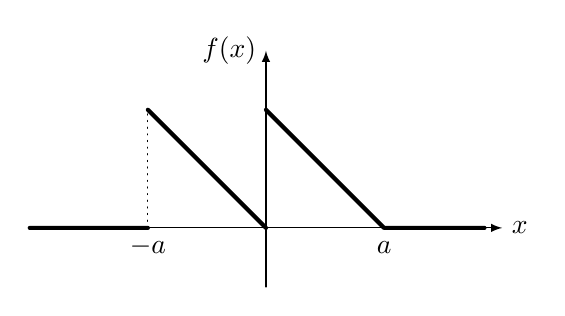
\begin{tikzpicture}[x = 1cm,		y = 1cm,		line join = round,		line cap = round,		> = latex, scale = 1.5,		]\draw[->]	(-2,0) -- (2,0)	node[right]	{$x$};\draw[->]	(0,-.5) --  (0,1.5)	node[left]	{$f(x)$};\draw[line width=1.5pt]		(-1,1) -- (0,0);\draw[line width=1.5pt]		(0,1) --  (1,0)				(-2,0) -- (-1,0)				(1,0) -- (1.85,0);\draw[dotted]		(-1,0) node[below] {$-a$} -- (-1,1);\draw[dotted]		(1,0)  node[below] {$\vphantom{-}a$} -- (1,0);\end{tikzpicture}\end{figure}
 
\end{zkrPlain}

\vfil

\begin{zkrPlain}{25}\noindent 
	Уровень воды в реке — случайная величина со средним значением $2{,}5$ м. Вероятность того, что в наудачу выбранный день уровень воды в реке окажется больше $3$ м, равна $0{,}62\%$. Найдите: \par \smallskip {\small \par \zz  вероятность того, что уровень воды в случайный день окажется в пределах от $240$ см до $270$ см;\par \zz $15\%$-ную точку этой случайной величины.}
 
\end{zkrPlain}

\vfil

\begin{zkrPlain}{25}\noindent 
	Вероятность сдачи в срок всех экзаменов студентом университета равна $ 0{,}07 $. Оцените вероятность того, что среди $ 750 $ студентов число сдавших в срок все экзамены отличается от своего математического ожидания не более чем на $ 27 $. 
 
\end{zkrPlain}

\newpage\setcounter{zad}{0}\setcounter{footnote}{0}



\begin{zkrPlain}{25}\noindent 
	Игральная кость подбрасывается до выпадения шестерки, но не более пяти раз. Случайная величина $X$ --- количество подбрасываний.  Найдите для этой случайной величины: \par \smallskip\small{ \par \zz ряд распределения (и постройте полигон); \par \zz функцию распределения (и постройте ее график); \par \zz математическое ожидание; \par \zz дисперсию и среднее квадратическое отклонение.\par \par}
 
\end{zkrPlain}

\vfil

\begin{zkrPlain}{25}\noindent 
	Найдите математическое ожидание, дисперсию и вероятность $P(X>a/2)$ непрерывной случайной величины с плотностью вероятностей $f(x)$, заданной графически\footnote{график может быть составлен лишь из участков прямых и парабол.}.\\ \begin{figure}[h!]\centering\small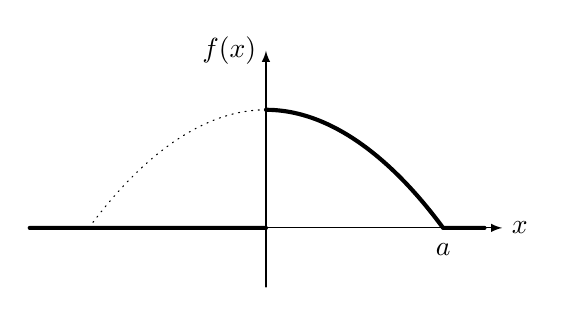
\begin{tikzpicture}[x = 1cm,		y = 1cm,		line join = round,		line cap = round,		> = latex, scale = 1.5,		]\draw[->]	(-2,0) -- (2,0)	node[right]	{$x$};\draw[->]	(0,-.5) --  (0,1.5)	node[left]	{$f(x)$};\draw[line width=1.5pt]	(0,1) parabola (1.5,0) node[below] {$\vphantom{-}a$}			(-2,0) -- (0,0)			(1.5,0) -- (1.85,0);\draw[dotted] (0,1) parabola (-1.5,0);\end{tikzpicture}\end{figure}
 
\end{zkrPlain}

\vfil

\begin{zkrPlain}{25}\noindent 
	Изменение индекса ценной бумаги на фондовой бирже может быть смоделировано как нормально распределенная случайная величина с параметром $\sigma^2 = 0{,}01$. Известно также, что на следующих торгах с вероятностью $0{,}0228$ изменение индекса будет менее $0{,}8$. Найдите: \par \smallskip {\small \par \zz вероятность того, что на следующих торгах изменение индекса будет больше $1{,}2$.\par \zz нижний квартиль ($x_{0{,}25}$) этой случайной величины.}
 
\end{zkrPlain}

\vfil

\begin{zkrPlain}{25}\noindent 
	Вероятность того, что акции, переданные на депозит, будут востребованы, равна $ 0{,}08 $. Оцените вероятность того, что среди $ 3200 $ клиентов от $ 197 $ до $ 315 $ востребуют свои акции.
 
\end{zkrPlain}

\newpage\setcounter{zad}{0}\setcounter{footnote}{0}



\begin{zkrPlain}{25}\noindent 
	Среди партии шарфов, поступивших в магазин, $70 \%$ составляют однотонные шарфы, а остальные --- пестрые. Покупатель из этих шарфов случайным образом выбирает три. Случайная величина $X$ --- количество пестрых шарфов в выборке.  Найдите для этой случайной величины: \par \smallskip\small{ \par \zz ряд распределения (и постройте полигон); \par \zz функцию распределения (и постройте ее график); \par \zz математическое ожидание; \par \zz дисперсию и среднее квадратическое отклонение.\par \par}
 
\end{zkrPlain}

\vfil

\begin{zkrPlain}{25}\noindent 
	Найдите математическое ожидание, дисперсию и вероятность $P(X>a/2)$ непрерывной случайной величины с плотностью вероятностей $f(x)$, заданной графически\footnote{график может быть составлен лишь из участков прямых и парабол.}.\\ \begin{figure}[h!]\centering\small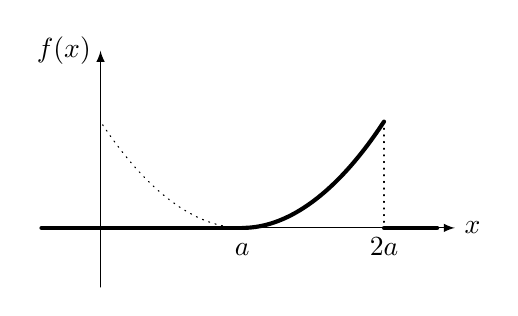
\begin{tikzpicture}[x = 1cm,		y = 1cm,		line join = round,		line cap = round,		> = latex, scale = 1.5,		]\draw[->]	(-.5,0) -- (3,0)	node[right]	{$x$};\draw[->]	(0,-.5) --  (0,1.5)	node[left]	{$f(x)$};\draw[line width=1.5pt]	(-.5,0) -- (1.2,0);\draw[line width=1.5pt]	(2.4,0) -- (2.85,0);\draw[line width=1.5pt]		(1.2,0) node[below] {$\vphantom{-}a$} parabola (2.4,.9);\draw[dotted]		(1.2,0) parabola (0,.9);\draw[dotted]	(2.4,.9) -- (2.4,0)  node[below] {$\vphantom{-}2a$};\end{tikzpicture}\end{figure}
 
\end{zkrPlain}

\vfil

\begin{zkrPlain}{25}\noindent 
	Сопротивление партии резисторов распределено по нормальному закону с номинальным средним значением $10$ кОм. Известно, что $84{,}13\%$ резисторов имеют сопротивление меньше $13$ кОм. Найдите: \par \smallskip {\small \par \zz вероятность того, что сопротивление выбранного наудачу резистора окажется в пределах от $9$ кОм до $11$ кОм;\par \zz с надежностью $90\%$ определить максимальное отклонение сопротивления от номинального среднего.}
 
\end{zkrPlain}

\vfil

\begin{zkrPlain}{25}\noindent 
	В течение времени $t$ экслуатируются $ 6500 $ приборов. Каждый прибор имеет надежность $ 0{,}5 $ и выходит из строя независимо от других. Оцените вероятность того, что в течение указанного времени выйдут из строя от $ 3098 $ до $ 3402 $ приборов.
 
\end{zkrPlain}

\newpage\setcounter{zad}{0}\setcounter{footnote}{0}



\begin{zkrPlain}{25}\noindent 
	Среди 15 монет 6 --- фальшивые. Наудачу вынимают пять монет. Случайная величина $X$ --- количество фальшивых монет в выборке.  Найдите для этой случайной величины: \par \smallskip\small{ \par \zz ряд распределения (и постройте полигон); \par \zz функцию распределения (и постройте ее график); \par \zz математическое ожидание; \par \zz дисперсию и среднее квадратическое отклонение.\par \par}
 
\end{zkrPlain}

\vfil

\begin{zkrPlain}{25}\noindent 
	Найдите математическое ожидание, дисперсию и вероятность $P(X>a/2)$ непрерывной случайной величины с плотностью вероятностей $f(x)$, заданной графически\footnote{график может быть составлен лишь из участков прямых и парабол.}.\\ \begin{figure}[h!]\centering\small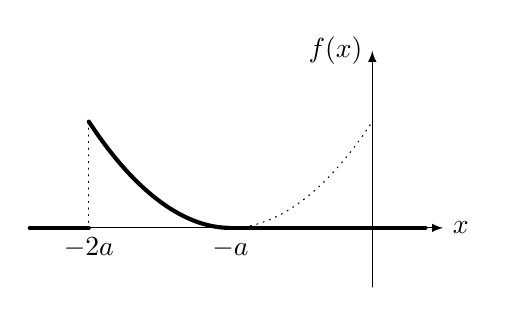
\begin{tikzpicture}[x = 1cm,		y = 1cm,		line join = round,		line cap = round,		> = latex, scale = 1.5,		]\draw[->]	(-.5,0) -- (3,0)	node[right]	{$x$};\draw[->]	(2.4,-.5) --  (2.4,1.5)	node[left]	{$f(x)$};\draw[line width=1.5pt]	(-.5,0) -- (0,0);\draw[line width=1.5pt]	(1.2,0) -- (2.85,0);\draw[dotted]		(1.2,0) parabola (2.4,.9);\draw[line width=1.5pt]		(1.2,0) node[below] {$-a$} parabola (0,.9);\draw[dotted]	(0,.9) -- (0,0) node[below] {$-2a$};\end{tikzpicture}\end{figure}
 
\end{zkrPlain}

\vfil

\begin{zkrPlain}{25}\noindent 
	Вес гигантского броненосца — нормально распределенная случайная величина. Известно, что $74{,}75\%$ этих животных в весе не превышают $27$ кг, а тяжелее $30$ кг — лишь $4{,}78\%$ броненосцев. Найдите: \par \smallskip {\small \par \zz вероятность случайно встретить в джунглях броненосца весом менее $22$ кг;\par \zz $9{,}12\%$-ную точку данной случайной величины.}
 
\end{zkrPlain}

\vfil

\begin{zkrPlain}{25}\noindent 
	Вероятность сдачи в срок всех экзаменов студентом университета равна $ 0{,}08 $. Оцените вероятность того, что среди $ 460 $ студентов число сдавших в срок все экзамены отличается от своего математического ожидания не более чем на $ 22 $. 
 
\end{zkrPlain}

\newpage\setcounter{zad}{0}\setcounter{footnote}{0}



\begin{zkrPlain}{25}\noindent 
	Экзаменатор задает студенту вопросы до тех пор, пока не получит верный ответ, но не более 3 вопросов. Вероятность того, что студент неверно ответит на первый вопрос, равна $6/7$ и с каждым последующим вопросом уменьшается на $1/7$. Случайная величина $X$ --- число вопросов, заданных студенту.  Найдите для этой случайной величины: \par \smallskip\small{ \par \zz ряд распределения (и постройте полигон); \par \zz функцию распределения (и постройте ее график); \par \zz математическое ожидание; \par \zz дисперсию и среднее квадратическое отклонение.\par \par}
 
\end{zkrPlain}

\vfil

\begin{zkrPlain}{25}\noindent 
	Найдите математическое ожидание, дисперсию и вероятность $P(X>a/2)$ непрерывной случайной величины с плотностью вероятностей $f(x)$, заданной графически\footnote{график может быть составлен лишь из участков прямых и парабол.}.\\ \begin{figure}[h!]\centering\small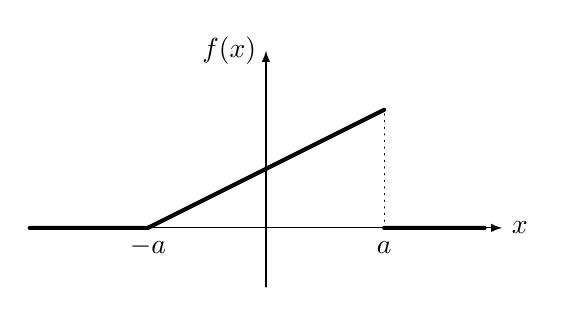
\begin{tikzpicture}[x = 1cm,		y = 1cm,		line join = round,		line cap = round,		> = latex, scale = 1.5,		]\draw[->]	(-2,0) -- (2,0)	node[right]	{$x$};\draw[->]	(0,-.5) --  (0,1.5)	node[left]	{$f(x)$};\draw[line width=1.5pt]		(-1,0) -- (1,1)				(-2,0) -- (-1,0)				(1,0) -- (1.85,0);\draw[dotted]		(-1,0) node[below] {$-a$} -- (-1,0);\draw[dotted]		(1,0)  node[below] {$\vphantom{-}a$} -- (1,1);\end{tikzpicture}\end{figure}
 
\end{zkrPlain}

\vfil

\begin{zkrPlain}{25}\noindent 
	Коробки с шоколадом упаковываются автоматически. Их средняя масса равна $1{,}2$ кг. Известно, что $9{,}68\%$ коробок имеют массу, меньшую $1{,}07$ кг. Предполагается, что масса коробки распределена нормально. Найдите: \par \smallskip {\small \par \zz процент коробок с массой, превышающей $1140$ г;\par \zz $30\%$-ную точку распределения.}
 
\end{zkrPlain}

\vfil

\begin{zkrPlain}{25}\noindent 
	Вероятность того, что акции, переданные на депозит, будут востребованы, равна $ 0{,}07 $. Оцените вероятность того, что среди $ 300 $ клиентов от $ 8 $ до $ 34 $ востребуют свои акции.
 
\end{zkrPlain}

\newpage\setcounter{zad}{0}\setcounter{footnote}{0}



\begin{zkrPlain}{25}\noindent 
		Противоположные грани кубика окрашены в красный, зеленый и синий цвета. Кубик подбрасывается 6 раз. Случайная величина $X$ --- количество подбрасываний, в результате которых сверху окажется грань, окрашенная в зеленый цвет.  Найдите для этой случайной величины: \par \smallskip\small{ \par \zz ряд распределения (и постройте полигон); \par \zz функцию распределения (и постройте ее график); \par \zz математическое ожидание; \par \zz дисперсию и среднее квадратическое отклонение.\par \par}
 
\end{zkrPlain}

\vfil

\begin{zkrPlain}{25}\noindent 
	Найдите математическое ожидание, дисперсию и вероятность $P(X>a/2)$ непрерывной случайной величины с плотностью вероятностей $f(x)$, заданной графически\footnote{график может быть составлен лишь из участков прямых и парабол.}.\\ \begin{figure}[h!]\centering\small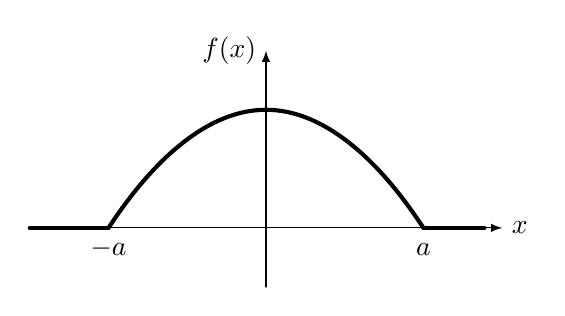
\begin{tikzpicture}[x = 1cm,		y = 1cm,		line join = round,		line cap = round,		> = latex, scale = 1.5,		]\draw[->]	(-2,0) -- (2,0)	node[right]	{$x$};\draw[->]	(0,-.5) --  (0,1.5)	node[left]	{$f(x)$};\draw[line width=1.5pt]		(0,1) parabola (4/3,0) node[below] {$\vphantom{-}a$};\draw[line width=1.5pt]		(0,1) parabola (-4/3,0) node[below] {$-a$};\draw[line width=1.5pt]		(-2,0) -- (-4/3,0)				(4/3,0) -- (1.85,0);\end{tikzpicture}\end{figure}
 
\end{zkrPlain}

\vfil

\begin{zkrPlain}{25}\noindent 
	Считаем, что рост императорского пингвина распределен нормально со средним квадратическим отклонением в три сантиметра. Известно, что $15{,}87\%$ императорских пингвинов имеют рост ниже $112$ см. Найдите: \par \smallskip {\small \par \zz долю императорских пингвинов с ростом от $116$ до $122$ см.;\par \zz с надежностью $0{,}9$ определить максимальное отклонение роста пингвина от его среднего значения.}
 
\end{zkrPlain}

\vfil

\begin{zkrPlain}{25}\noindent 
	Электростанция обслуживает сеть на $ 7000 $ электроламп, вероятность включения которых утром равна $ 0{,}6 $. Оцените вероятность того, что число ламп, включенных в сеть сегодня утром, отличается от своего математического ожидания более чем на $ 96 $ (по абсолютной величине). 
 
\end{zkrPlain}

\newpage\setcounter{zad}{0}\setcounter{footnote}{0}



\begin{zkrPlain}{25}\noindent 
	В корзине 7 синих и 6 красных мячей. Наудачу вынимают четыре мяча. Случайная величина $X$ --- количество красных мячей в выборке.  Найдите для этой случайной величины: \par \smallskip\small{ \par \zz ряд распределения (и постройте полигон); \par \zz функцию распределения (и постройте ее график); \par \zz математическое ожидание; \par \zz дисперсию и среднее квадратическое отклонение.\par \par}
 
\end{zkrPlain}

\vfil

\begin{zkrPlain}{25}\noindent 
	Найдите математическое ожидание, дисперсию и вероятность $P(X>a/2)$ непрерывной случайной величины с плотностью вероятностей $f(x)$, заданной графически\footnote{график может быть составлен лишь из участков прямых и парабол.}.\\ \begin{figure}[h!]\centering\small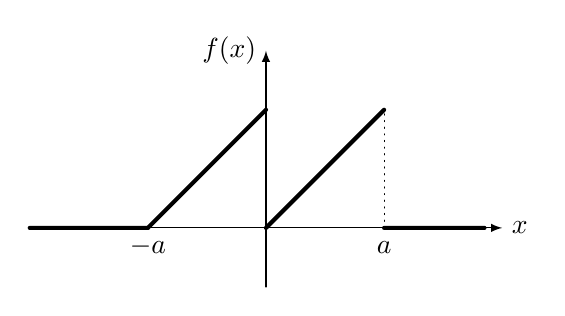
\begin{tikzpicture}[x = 1cm,		y = 1cm,		line join = round,		line cap = round,		> = latex, scale = 1.5,		]\draw[->]	(-2,0) -- (2,0)	node[right]	{$x$};\draw[->]	(0,-.5) --  (0,1.5)	node[left]	{$f(x)$};\draw[line width=1.5pt]		(-1,0) -- (0,1);\draw[line width=1.5pt]		(0,0)  --  (1,1)				(-2,0) -- (-1,0)				(1,0) -- (1.85,0);\draw[dotted]		(-1,0) node[below] {$-a$} -- (-1,0);\draw[dotted]		(1,0)  node[below] {$\vphantom{-}a$} -- (1,1);\end{tikzpicture}\end{figure}
 
\end{zkrPlain}

\vfil

\begin{zkrPlain}{25}\noindent 
	Длина переднего рога у африканского белого носорога распределена по нормальному закону с параметром $\sigma = 5$ (см). Всего лишь $2{,}28\%$ белых носорогов имеют рог длиной более $100$ см. Найдите: \par \smallskip {\small \par \zz долю носорогов с рогом длиной от $85$ см до $95$ см;\par \zz квантиль уровня $0{,}3$.}
 
\end{zkrPlain}

\vfil

\begin{zkrPlain}{25}\noindent 
	В течение времени $t$ экслуатируются $ 330 $ приборов. Каждый прибор имеет надежность $ 0{,}7 $ и выходит из строя независимо от других. Оцените вероятность того, что в течение указанного времени выйдут из строя от $ 222 $ до $ 240 $ приборов.
 
\end{zkrPlain}

\newpage\setcounter{zad}{0}\setcounter{footnote}{0}



\begin{zkrPlain}{25}\noindent 
	Из букв слова СТАТИСТИКА случайным образом выбирают 4 буквы. Случайная величина $X$--- количество гласных букв в выборке. Найдите для этой случайной величины: \par \smallskip\small{ \par \zz ряд распределения (и постройте полигон); \par \zz функцию распределения (и постройте ее график); \par \zz математическое ожидание; \par \zz дисперсию и среднее квадратическое отклонение.\par \par}
 
\end{zkrPlain}

\vfil

\begin{zkrPlain}{25}\noindent 
	Найдите математическое ожидание, дисперсию и вероятность $P(X>a/2)$ непрерывной случайной величины с плотностью вероятностей $f(x)$, заданной графически\footnote{график может быть составлен лишь из участков прямых и парабол.}.\\ \begin{figure}[h!]\centering\small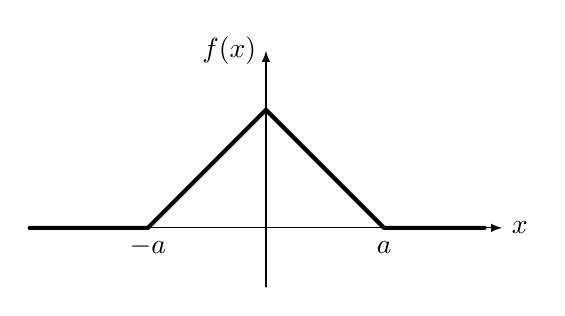
\begin{tikzpicture}[x = 1cm,		y = 1cm,		line join = round,		line cap = round,		> = latex, scale = 1.5,		]\draw[->]	(-2,0) -- (2,0)	node[right]	{$x$};\draw[->]	(0,-.5) --  (0,1.5)	node[left]	{$f(x)$};\draw[line width=1.5pt]		(-1,0) -- (0,1) --  (1,0)				(-2,0) -- (-1,0)				(1,0) -- (1.85,0);\draw[dotted]		(-1,0) node[below] {$-a$} -- (-1,0);\draw[dotted]		(1,0)  node[below] {$\vphantom{-}a$} -- (1,0);\end{tikzpicture}\end{figure}
 
\end{zkrPlain}

\vfil

\begin{zkrPlain}{25}\noindent 
	Средний рост представителя пигмейских народов гиелли и эфе равен $147$ см. Известно также, что «высоких» людей (выше $1{,}5$ м) среди этих народов — лишь $0{,}13\%$. Учесть, что рост человека (хотя бы и пигмея) распределен нормально. Найдите: \par \smallskip {\small \par \zz долю пигмеев, имеющих рост от $146$ до $148$ см ;\par \zz квантиль уровня $0{,}0227$ описанной случайной величины.}
 
\end{zkrPlain}

\vfil

\begin{zkrPlain}{25}\noindent 
	Среднее значение длины детали $ 27 $ см, а дисперсия --- $ 25 $. Оцените вероятность того, что случайно взятая деталь окажется по длине не менее $ 20 $ и не более $ 34 $ см.
 
\end{zkrPlain}

\newpage\setcounter{zad}{0}\setcounter{footnote}{0}



\begin{zkrPlain}{25}\noindent 
	На экзамен пришли пять студентов, уровень подготовки которых примерно одинаков. Вероятность того, что каждый студент завалит экзамен, равна $40\%$ и не зависит от результатов сдачи остальных. Случайная величина $X$ --- число студентов, заваливших экзамен.  Найдите для этой случайной величины: \par \smallskip\small{ \par \zz ряд распределения (и постройте полигон); \par \zz функцию распределения (и постройте ее график); \par \zz математическое ожидание; \par \zz дисперсию и среднее квадратическое отклонение.\par \par}
 
\end{zkrPlain}

\vfil

\begin{zkrPlain}{25}\noindent 
	Найдите математическое ожидание, дисперсию и вероятность $P(X>a/2)$ непрерывной случайной величины с плотностью вероятностей $f(x)$, заданной графически\footnote{график может быть составлен лишь из участков прямых и парабол.}.\\ \begin{figure}[h!]\centering\small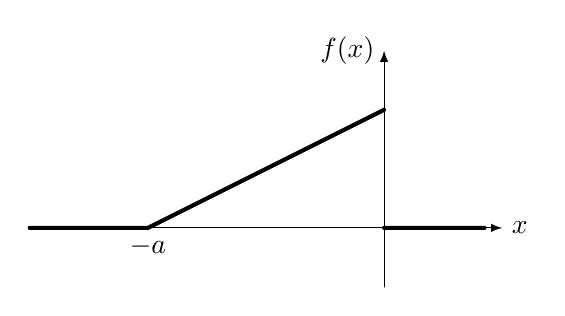
\begin{tikzpicture}[x = 1cm,		y = 1cm,		line join = round,		line cap = round,		> = latex, scale = 1.5,		]\draw[->]	(-3,0) -- (1,0)	node[right]	{$x$};\draw[->]	(0,-.5) --  (0,1.5)	node[left]	{$f(x)$};\draw[line width=1.5pt]		(-2,0) -- (0,1)				(-3,0) -- (-2,0)				(0,0) -- (.85,0);\draw[dotted]		(-2,0) node[below] {$-a$} -- (-2,0);\end{tikzpicture}\end{figure}
 
\end{zkrPlain}

\vfil

\begin{zkrPlain}{25}\noindent 
	Вес рыб, обитающих в водоеме, подчиняется нормальному закону с параметром $a = 375$ г. Вероятность того, что вес пойманной рыбы меньше $400$ г, равна $0{,}8413$. Найдите: \par \smallskip {\small \par \zz вероятность того, что вес выловленной наудачу рыбы попадет в промежуток от $300$ г до $425$ г;\par \zz квантиль уровня $0{,}7$.}
 
\end{zkrPlain}

\vfil

\begin{zkrPlain}{25}\noindent 
	В среднем $ 7 \% $ работоспособного населения некоторого региона --- безработные. Оцените вероятность того, что уровень безработицы среди обследованных $ 2300 $ работоспособных жителей города будет в пределах от $ 5 \% $ до $ 9 \% $.
 
\end{zkrPlain}

\newpage\setcounter{zad}{0}\setcounter{footnote}{0}



\begin{zkrPlain}{25}\noindent 
	На маршруте работают три автобуса. Вероятность поломки каждого из них в течение рабочего дня равна $0{,}1$ и не зависит от состояния остальных. Случайная величина $X$ --- число неисправных в течение рабочего дня автобусов.  Найдите для этой случайной величины: \par \smallskip\small{ \par \zz ряд распределения (и постройте полигон); \par \zz функцию распределения (и постройте ее график); \par \zz математическое ожидание; \par \zz дисперсию и среднее квадратическое отклонение.\par \par}
 
\end{zkrPlain}

\vfil

\begin{zkrPlain}{25}\noindent 
	Найдите математическое ожидание, дисперсию и вероятность $P(X>a/2)$ непрерывной случайной величины с плотностью вероятностей $f(x)$, заданной графически\footnote{график может быть составлен лишь из участков прямых и парабол.}.\\ \begin{figure}[h!]\centering\small\begin{tikzpicture}[x = 1cm,		y = 1cm,		line join = round,		line cap = round,		> = latex, scale = 1.5,		]\draw[->]	(-.5,0) -- (3,0)	node[right]	{$x$};\draw[->]	(0,-.5) --  (0,1.5)	node[left]	{$f(x)$};\draw[line width=1.5pt]	(-.5,0) -- (0,0);\draw[line width=1.5pt]	(1.2,0) -- (2.85,0);\draw[dotted]		(1.2,0) parabola (2.4,.9);\draw[line width=1.5pt]		(1.2,0) parabola (0,.9);\draw[dotted]	(1.2,0) -- (1.2,0) node[below]	{$\vphantom{-}a$};\end{tikzpicture}\end{figure}
 
\end{zkrPlain}

\vfil

\begin{zkrPlain}{25}\noindent 
	Средний вес расфасованных пакетов со стиральным порошком $930$ г, но, как правило, около $6{,}68\%$ пакетов тяжелее $960$ г. Считаем, что вес пакетов распределен нормально. Найдите: \par \smallskip {\small \par \zz долю пакетов, имеющих вес до $900$ г.\par \zz Требуется, чтобы не более $4\%$ пакетов содержали меньше $900$ г порошка. На какой средний вес пакетов нужно переналадить фасовочный автомат для выполнения этого задания?}
 
\end{zkrPlain}

\vfil

\begin{zkrPlain}{25}\noindent 
	Электростанция обслуживает сеть на $ 200 $ электроламп, вероятность включения которых утром равна $ 0{,}7 $. Оцените вероятность того, что число ламп, включенных в сеть сегодня утром, отличается от своего математического ожидания более чем на $ 18 $ (по абсолютной величине). 
 
\end{zkrPlain}

\newpage\setcounter{zad}{0}\setcounter{footnote}{0}



\begin{zkrPlain}{25}\noindent 
	Вероятность заболеть гриппом в период эпидемии составляет $0{,}1$. Рассматривается контрольная группа, состоящая из пяти человек. Случайная величина $X$ --- количество заболевших в период эпидемии человек данной группы.  Найдите для этой случайной величины: \par \smallskip\small{ \par \zz ряд распределения (и постройте полигон); \par \zz функцию распределения (и постройте ее график); \par \zz математическое ожидание; \par \zz дисперсию и среднее квадратическое отклонение.\par \par}
 
\end{zkrPlain}

\vfil

\begin{zkrPlain}{25}\noindent 
	Найдите математическое ожидание, дисперсию и вероятность $P(X>a/2)$ непрерывной случайной величины с плотностью вероятностей $f(x)$, заданной графически\footnote{график может быть составлен лишь из участков прямых и парабол.}.\\ \begin{figure}[h!]\centering\small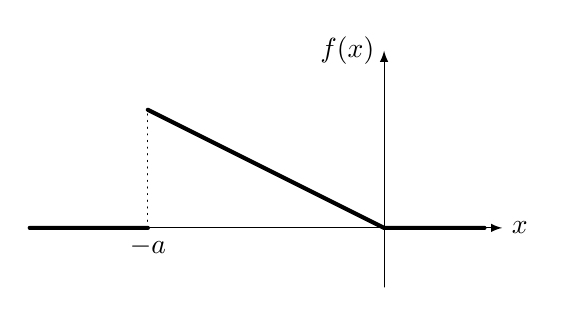
\begin{tikzpicture}[x = 1cm,		y = 1cm,		line join = round,		line cap = round,		> = latex, scale = 1.5,		]\draw[->]	(-3,0) -- (1,0)	node[right]	{$x$};\draw[->]	(0,-.5) --  (0,1.5)	node[left]	{$f(x)$};\draw[line width=1.5pt]		(-2,1) -- (0,0)				(-3,0) -- (-2,0)				(0,0) -- (.85,0);\draw[dotted]		(-2,0) node[below] {$-a$} -- (-2,1);\end{tikzpicture}\end{figure}
 
\end{zkrPlain}

\vfil

\begin{zkrPlain}{25}\noindent 
	Словарный запас английского языка у изучающих его — случайная величина, распределенная нормально. Известно, что в среднем этот запас составляет 8000 слов. Кроме этого, имеются данные, согласно которым $30{,}85\%$ изучающих имеют словарный запас менее $6000$ слов. Найдите: \par \smallskip {\small \par \zz долю изучающих английский со словарным запасом более $15000$ слов;\par \zz нижний квартиль ($x_{0{,}25}$)указанной случайной величины.}
 
\end{zkrPlain}

\vfil

\begin{zkrPlain}{25}\noindent 
	В среднем $ 7 \% $ работоспособного населения некоторого региона --- безработные. Оцените вероятность того, что уровень безработицы среди обследованных $ 690 $ работоспособных жителей города будет в пределах от $ 5 \% $ до $ 9 \% $.
 
\end{zkrPlain}

\newpage\setcounter{zad}{0}\setcounter{footnote}{0}



\begin{zkrPlain}{25}\noindent 
	В контрольной работе шесть задач. Вероятность правильного решения студентом каждой задачи равна $0{,}9$ и не зависит от правильности решения остальных. Случайная величина $X$ --- количество правильно решенных задач.  Найдите для этой случайной величины: \par \smallskip\small{ \par \zz ряд распределения (и постройте полигон); \par \zz функцию распределения (и постройте ее график); \par \zz математическое ожидание; \par \zz дисперсию и среднее квадратическое отклонение.\par \par}
 
\end{zkrPlain}

\vfil

\begin{zkrPlain}{25}\noindent 
	Найдите математическое ожидание, дисперсию и вероятность $P(X>a/2)$ непрерывной случайной величины с плотностью вероятностей $f(x)$, заданной графически\footnote{график может быть составлен лишь из участков прямых и парабол.}.\\ \begin{figure}[h!]\centering\small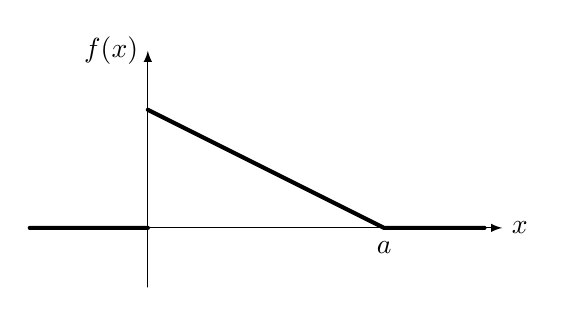
\begin{tikzpicture}[x = 1cm,		y = 1cm,		line join = round,		line cap = round,		> = latex, scale = 1.5,		]\draw[->]	(-1,0) -- (3,0)	node[right]	{$x$};\draw[->]	(0,-.5) --  (0,1.5)	node[left]	{$f(x)$};\draw[line width=1.5pt]		 (0,1) --  (2,0)				(-1,0) -- (0,0)				(2,0) -- (2.85,0);\draw[dotted]		(2,0)  node[below] {$\vphantom{-}a$} -- (2,0);\end{tikzpicture}\end{figure}
 
\end{zkrPlain}

\vfil

\begin{zkrPlain}{25}\noindent 
	Средняя высота секвойи вечнозеленой  — порядка {$90$~м}. Примерно $1{,}31\%$ этих деревьев достигают в высоту $110$~м и более. Будем считать, что высота секвойи — нормально распределенная случайная величина. Найдите: \par \smallskip {\small \par \zz вероятность обнаружить секвойю высотой от $95$ до $105$ м;\par \zz вероятность того, что отклонение высоты случайной секвойи от средней составит не более десяти метров (по абсолютной величине).}
 
\end{zkrPlain}

\vfil

\begin{zkrPlain}{25}\noindent 
	Среднее значение длины детали $ 427 $ см, а дисперсия --- $ 397 $. Оцените вероятность того, что случайно взятая деталь окажется по длине не менее $ 350 $ и не более $ 504 $ см.
 
\end{zkrPlain}

\newpage\setcounter{zad}{0}\setcounter{footnote}{0}



\begin{zkrPlain}{25}\noindent 
	В кошельке 4 двухрублевые и 3 пятирублевые монеты. Наудачу извлекают пять монет. Случайная величина $X$ --- сумма денег в рублях, которую составляют извлеченные монеты.  Найдите для этой случайной величины: \par \smallskip\small{ \par \zz ряд распределения (и постройте полигон); \par \zz функцию распределения (и постройте ее график); \par \zz математическое ожидание; \par \zz дисперсию и среднее квадратическое отклонение.\par \par}
 
\end{zkrPlain}

\vfil

\begin{zkrPlain}{25}\noindent 
	Найдите математическое ожидание, дисперсию и вероятность $P(X>a/2)$ непрерывной случайной величины с плотностью вероятностей $f(x)$, заданной графически\footnote{график может быть составлен лишь из участков прямых и парабол.}.\\ \begin{figure}[h!]\centering\small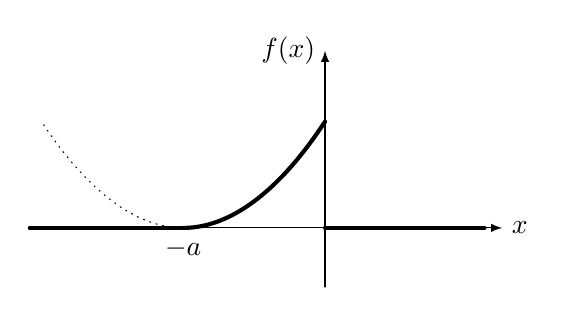
\begin{tikzpicture}[x = 1cm,		y = 1cm,		line join = round,		line cap = round,		> = latex, scale = 1.5,		]\draw[->]	(-2.5,0) -- (1.5,0)	node[right]	{$x$};\draw[->]	(0,-.5) --  (0,1.5)	node[left]	{$f(x)$};\draw[line width=1.5pt]		(-1.2,0) node[below] {$-a$} parabola (0,.9);\draw[line width=1.5pt]		(-2.5,0) -- (-1.2,0)				(0,0) -- (1.35,0);\draw[dotted]	(-1.2,0) parabola (-2.4,.9);\end{tikzpicture}\end{figure}
 
\end{zkrPlain}

\vfil

\begin{zkrPlain}{25}\noindent 
	Отклонение количества изюма в кексах от среднего больше $15$ изюмин на кекс встречается в $68{,}27\%$ кексов. Кроме этого, замечено, что в $25{,}25\%$ случаев число изюминок в кексе меньше $70$. Найдите: \par \smallskip {\small \par \zz вероятность того, что изюминок в купленном кексе окажется от $90$ до $100$;\par \zz $4{,}78\%$-ную точку числа изюмин.}
 
\end{zkrPlain}

\vfil

\begin{zkrPlain}{25}\noindent 
	В течение времени $t$ экслуатируются $ 7200 $ приборов. Каждый прибор имеет надежность $ 0{,}8 $ и выходит из строя независимо от других. Оцените вероятность того, что в течение указанного времени выйдут из строя от $ 5680 $ до $ 5840 $ приборов.
 
\end{zkrPlain}

\newpage\setcounter{zad}{0}\setcounter{footnote}{0}



\begin{zkrPlain}{25}\noindent 
	Стрелок ведет стрельбу по цели с вероятностью промаха при каждом выстреле $85\%$. За каждое попадание он получает 10 очков, а в случае промаха очков ему не начисляют. Случайная величина $X$ --- число очков, полученных стрелком за 4 выстрелов.  Найдите для этой случайной величины: \par \smallskip\small{ \par \zz ряд распределения (и постройте полигон); \par \zz функцию распределения (и постройте ее график); \par \zz математическое ожидание; \par \zz дисперсию и среднее квадратическое отклонение.\par \par}
 
\end{zkrPlain}

\vfil

\begin{zkrPlain}{25}\noindent 
	Найдите математическое ожидание, дисперсию и вероятность $P(X>a/2)$ непрерывной случайной величины с плотностью вероятностей $f(x)$, заданной графически\footnote{график может быть составлен лишь из участков прямых и парабол.}.\\ \begin{figure}[h!]\centering\small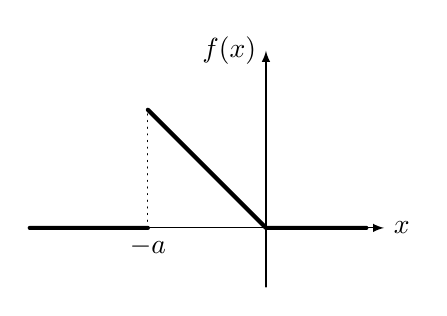
\begin{tikzpicture}[x = 1cm,		y = 1cm,		line join = round,		line cap = round,		> = latex, scale = 1.5,		]\draw[->]	(-2,0) -- (1,0)	node[right]	{$x$};\draw[->]	(0,-.5) --  (0,1.5)	node[left]	{$f(x)$};\draw[line width=1.5pt]		(-1,1) -- (0,0)				(-2,0) -- (-1,0)				(0,0) -- (.85,0);\draw[dotted]		(-1,0) node[below] {$-a$} -- (-1,1);\end{tikzpicture}\end{figure}
 
\end{zkrPlain}

\vfil

\begin{zkrPlain}{25}\noindent 
	Спортсмен бросает копье. Дальность полета — нормально распределенная величина со средним значением $70$ м. По статистике $2{,}28\%$ бросков, как правило, оказываются неудачными (дальность полета менее $60$ м).  Найдите: \par \smallskip {\small \par \zz  вероятность того, что копье упадет на расстоянии от $65$ м до $75$ м.\par \zz нижний квартиль распределения ($x_{0{,}25}$).}
 
\end{zkrPlain}

\vfil

\begin{zkrPlain}{25}\noindent 
	Вероятность того, что акции, переданные на депозит, будут востребованы, равна $ 0{,}05 $. Оцените вероятность того, что среди $ 420 $ клиентов от $ 4 $ до $ 38 $ востребуют свои акции.
 
\end{zkrPlain}

\newpage\setcounter{zad}{0}\setcounter{footnote}{0}



\begin{zkrPlain}{25}\noindent 
	Экзаменатор задает студенту вопросы до тех пор, пока не получит неверный ответ, но не более 3 вопросов. Вероятность того, что студент верно ответит на первый вопрос, равна $1/8$ и с каждым последующим вопросом увеличивается на $1/8$. Случайная величина $X$ --- число вопросов, заданных студенту.  Найдите для этой случайной величины: \par \smallskip\small{ \par \zz ряд распределения (и постройте полигон); \par \zz функцию распределения (и постройте ее график); \par \zz математическое ожидание; \par \zz дисперсию и среднее квадратическое отклонение.\par \par}
 
\end{zkrPlain}

\vfil

\begin{zkrPlain}{25}\noindent 
	Найдите математическое ожидание, дисперсию и вероятность $P(X>a/2)$ непрерывной случайной величины с плотностью вероятностей $f(x)$, заданной графически\footnote{график может быть составлен лишь из участков прямых и парабол.}.\\ \begin{figure}[h!]\centering\small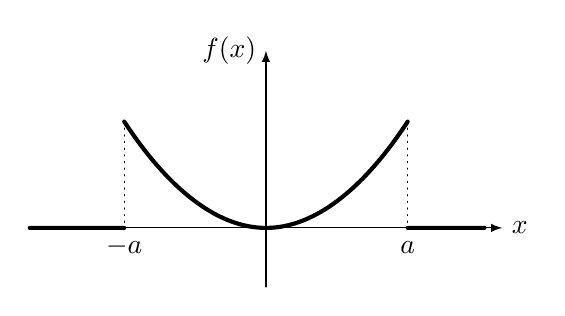
\begin{tikzpicture}[x = 1cm,		y = 1cm,		line join = round,		line cap = round,		> = latex, scale = 1.5,		]\draw[->]	(-2,0) -- (2,0)	node[right]	{$x$};\draw[->]	(0,-.5) --  (0,1.5)	node[left]	{$f(x)$};\draw[line width=1.5pt]		(0,0) parabola (1.2,.9);\draw[line width=1.5pt]		(0,0) parabola (-1.2,.9)				(-2,0) -- (-1.2,0)				(1.2,0) -- (1.85,0);\draw[dotted]	(-1.2,.9) -- (-1.2,0) node[below]	{$-a$};\draw[dotted]	(1.2,.9) -- (1.2,0) node[below]	{$\vphantom{-}a$};\end{tikzpicture}\end{figure}
 
\end{zkrPlain}

\vfil

\begin{zkrPlain}{25}\noindent 
	По статистике ЕГЭ-2012 (русский язык), $7{,}66\%$ выпускников набрали менее $40$ баллов. Известно также, что $23{,}75\%$ выпускников получили более $70$ баллов. Считаем распределение баллов нормальным. Найдите: \par \smallskip {\small \par \zz средний балл по русскому языку;\par \zz долю отличников, получивших более $90$ баллов.}
 
\end{zkrPlain}

\vfil

\begin{zkrPlain}{25}\noindent 
	Вероятность сдачи в срок всех экзаменов студентом университета равна $ 0{,}06 $. Оцените вероятность того, что среди $ 2000 $ студентов число сдавших в срок все экзамены отличается от своего математического ожидания не более чем на $ 13 $. 
 
\end{zkrPlain}

\newpage\setcounter{zad}{0}\setcounter{footnote}{0}



\begin{zkrPlain}{25}\noindent 
	В ящике находятся 12 деталей, среди которых 5 бракованные. Наудачу из этих деталей вынимаются 4. Случайная величина $X$ --- количество бракованных деталей в выборке.  Найдите для этой случайной величины: \par \smallskip\small{ \par \zz ряд распределения (и постройте полигон); \par \zz функцию распределения (и постройте ее график); \par \zz математическое ожидание; \par \zz дисперсию и среднее квадратическое отклонение.\par \par}
 
\end{zkrPlain}

\vfil

\begin{zkrPlain}{25}\noindent 
	Найдите математическое ожидание, дисперсию и вероятность $P(X>a/2)$ непрерывной случайной величины с плотностью вероятностей $f(x)$, заданной графически\footnote{график может быть составлен лишь из участков прямых и парабол.}.\\ \begin{figure}[h!]\centering\small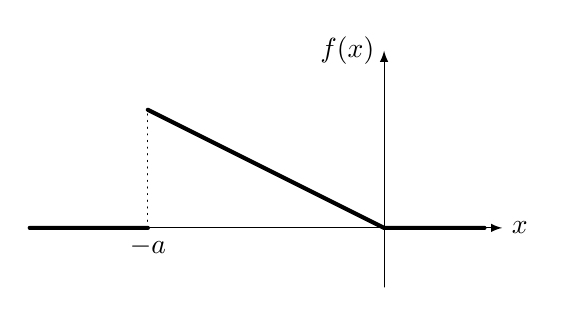
\begin{tikzpicture}[x = 1cm,		y = 1cm,		line join = round,		line cap = round,		> = latex, scale = 1.5,		]\draw[->]	(-3,0) -- (1,0)	node[right]	{$x$};\draw[->]	(0,-.5) --  (0,1.5)	node[left]	{$f(x)$};\draw[line width=1.5pt]		(-2,1) -- (0,0)				(-3,0) -- (-2,0)				(0,0) -- (.85,0);\draw[dotted]		(-2,0) node[below] {$-a$} -- (-2,1);\end{tikzpicture}\end{figure}
 
\end{zkrPlain}

\vfil

\begin{zkrPlain}{25}\noindent 
	Тесты IQ разрабатываются так, чтобы их результаты описывались нормальным распределением со средним значением $100$ и с таким разбросом, чтобы $25\%$ тестируемых имели IQ ниже $90$. Найдите: \par \smallskip {\small \par \zz вероятность случайному испытуемому получить по результатам теста IQ от $110$  до $120$;\par \zz с помощью правила трех сигм границы, в которых находится IQ большинства людей.}
 
\end{zkrPlain}

\vfil

\begin{zkrPlain}{25}\noindent 
	В среднем $ 5 \% $ работоспособного населения некоторого региона --- безработные. Оцените вероятность того, что уровень безработицы среди обследованных $ 800 $ работоспособных жителей города будет в пределах от $ 2 \% $ до $ 8 \% $.
 
\end{zkrPlain}

\newpage\setcounter{zad}{0}\setcounter{footnote}{0}



\begin{zkrPlain}{25}\noindent 
	Секретариат фирмы оборудован четырьмя независимо работающими компьютерами. Вероятность отказа каждого из них в течение рабочего дня равна $70\%$. Случайная величина $X$ --- количество отказавших в течение рабочего дня компьютеров.  Найдите для этой случайной величины: \par \smallskip\small{ \par \zz ряд распределения (и постройте полигон); \par \zz функцию распределения (и постройте ее график); \par \zz математическое ожидание; \par \zz дисперсию и среднее квадратическое отклонение.\par \par}
 
\end{zkrPlain}

\vfil

\begin{zkrPlain}{25}\noindent 
	Найдите математическое ожидание, дисперсию и вероятность $P(X>a/2)$ непрерывной случайной величины с плотностью вероятностей $f(x)$, заданной графически\footnote{график может быть составлен лишь из участков прямых и парабол.}.\\ \begin{figure}[h!]\centering\small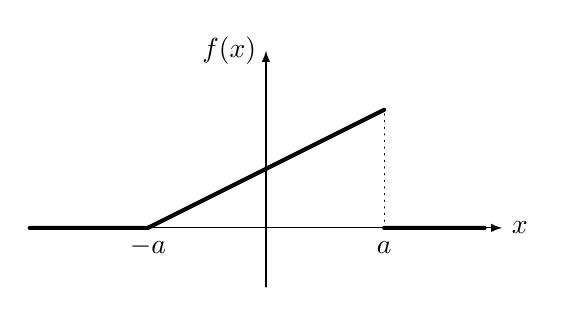
\begin{tikzpicture}[x = 1cm,		y = 1cm,		line join = round,		line cap = round,		> = latex, scale = 1.5,		]\draw[->]	(-2,0) -- (2,0)	node[right]	{$x$};\draw[->]	(0,-.5) --  (0,1.5)	node[left]	{$f(x)$};\draw[line width=1.5pt]		(-1,0) -- (1,1)				(-2,0) -- (-1,0)				(1,0) -- (1.85,0);\draw[dotted]		(-1,0) node[below] {$-a$} -- (-1,0);\draw[dotted]		(1,0)  node[below] {$\vphantom{-}a$} -- (1,1);\end{tikzpicture}\end{figure}
 
\end{zkrPlain}

\vfil

\begin{zkrPlain}{25}\noindent 
	Прочность пряжи приблизительно следует нормальному закону распределения. Средняя прочность пряжи — $245$ сн\footnote{1 сн (стен [тэ]) = 1000 ньютонов}. $1{,}22\%$ пряжи имеет прочность менее $200$ сн. Найдите: \par \smallskip {\small \par \zz вероятность того, что прочность окажется в интервале от $220$ сн до $270$ сн.\par \zz оценить наиболее вероятные границы прочности с помощью правила трех сигм.}
 
\end{zkrPlain}

\vfil

\begin{zkrPlain}{25}\noindent 
	Электростанция обслуживает сеть на $ 5200 $ электроламп, вероятность включения которых утром равна $ 0{,}6 $. Оцените вероятность того, что число ламп, включенных в сеть сегодня утром, отличается от своего математического ожидания более чем на $ 109 $ (по абсолютной величине). 
 
\end{zkrPlain}

\newpage\setcounter{zad}{0}\setcounter{footnote}{0}



\begin{zkrPlain}{25}\noindent 
	Сотрудник лаборатории проводит пять независимых опытов. Вероятность успешного опыта равна $3/8$ и не зависит от успешности предыдущих опытов. Случайная величина $X$ --- число неудачных опытов.  Найдите для этой случайной величины: \par \smallskip\small{ \par \zz ряд распределения (и постройте полигон); \par \zz функцию распределения (и постройте ее график); \par \zz математическое ожидание; \par \zz дисперсию и среднее квадратическое отклонение.\par \par}
 
\end{zkrPlain}

\vfil

\begin{zkrPlain}{25}\noindent 
	Найдите математическое ожидание, дисперсию и вероятность $P(X>a/2)$ непрерывной случайной величины с плотностью вероятностей $f(x)$, заданной графически\footnote{график может быть составлен лишь из участков прямых и парабол.}.\\ \begin{figure}[h!]\centering\small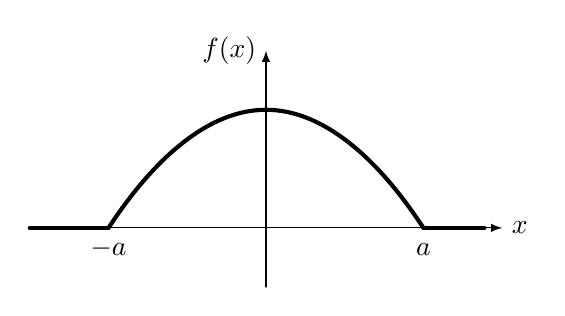
\begin{tikzpicture}[x = 1cm,		y = 1cm,		line join = round,		line cap = round,		> = latex, scale = 1.5,		]\draw[->]	(-2,0) -- (2,0)	node[right]	{$x$};\draw[->]	(0,-.5) --  (0,1.5)	node[left]	{$f(x)$};\draw[line width=1.5pt]		(0,1) parabola (4/3,0) node[below] {$\vphantom{-}a$};\draw[line width=1.5pt]		(0,1) parabola (-4/3,0) node[below] {$-a$};\draw[line width=1.5pt]		(-2,0) -- (-4/3,0)				(4/3,0) -- (1.85,0);\end{tikzpicture}\end{figure}
 
\end{zkrPlain}

\vfil

\begin{zkrPlain}{25}\noindent 
	Максимальная урожайность большей части современных сортов картофеля — нормально распределенная случайная величина, принимающая $99{,}73\%$ своих значений в интервале $420-780$ ц/га. Найдите: \par \smallskip {\small \par \zz вероятность того, что урожайность высаженного картофеля в данном году составит от $650$ до $700$ ц/га;\par \zz $36{,}94\%$-ную точку указанной случайной величины.}
 
\end{zkrPlain}

\vfil

\begin{zkrPlain}{25}\noindent 
	В течение времени $t$ экслуатируются $ 600 $ приборов. Каждый прибор имеет надежность $ 0{,}5 $ и выходит из строя независимо от других. Оцените вероятность того, что в течение указанного времени выйдут из строя от $ 273 $ до $ 327 $ приборов.
 
\end{zkrPlain}

\newpage\setcounter{zad}{0}\setcounter{footnote}{0}



\begin{zkrPlain}{25}\noindent 
	Всхожесть семян данного сорта растений равна $0{,}1$. Посеяно пять семян. Случайная величина $X$ --- количество невзошедших семян из посеянных. Найдите для этой случайной величины: \par \smallskip\small{ \par \zz ряд распределения (и постройте полигон); \par \zz функцию распределения (и постройте ее график); \par \zz математическое ожидание; \par \zz дисперсию и среднее квадратическое отклонение.\par \par}
 
\end{zkrPlain}

\vfil

\begin{zkrPlain}{25}\noindent 
	Найдите математическое ожидание, дисперсию и вероятность $P(X>a/2)$ непрерывной случайной величины с плотностью вероятностей $f(x)$, заданной графически\footnote{график может быть составлен лишь из участков прямых и парабол.}.\\ \begin{figure}[h!]\centering\small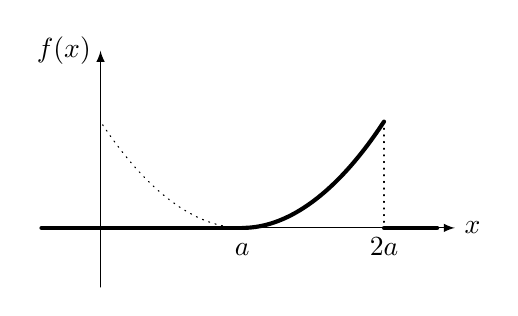
\begin{tikzpicture}[x = 1cm,		y = 1cm,		line join = round,		line cap = round,		> = latex, scale = 1.5,		]\draw[->]	(-.5,0) -- (3,0)	node[right]	{$x$};\draw[->]	(0,-.5) --  (0,1.5)	node[left]	{$f(x)$};\draw[line width=1.5pt]	(-.5,0) -- (1.2,0);\draw[line width=1.5pt]	(2.4,0) -- (2.85,0);\draw[line width=1.5pt]		(1.2,0) node[below] {$\vphantom{-}a$} parabola (2.4,.9);\draw[dotted]		(1.2,0) parabola (0,.9);\draw[dotted]	(2.4,.9) -- (2.4,0)  node[below] {$\vphantom{-}2a$};\end{tikzpicture}\end{figure}
 
\end{zkrPlain}

\vfil

\begin{zkrPlain}{25}\noindent 
	Вес товаров, помещаемых в контейнер определенного размера, — нормально распределенная случайная величина. Известно, что $34{,}46\%$ контейнеров имеют чистый вес меньше $8$ тонн и $21{,}19\%$ имеют вес больше, чем $14$ тонн. Найдите: \par \smallskip {\small \par \zz средний вес одного контейнера; \par \zz с надежностью $0{,}9$ максимальное отклонение веса контейнера от среднего значения. }
 
\end{zkrPlain}

\vfil

\begin{zkrPlain}{25}\noindent 
	Вероятность того, что акции, переданные на депозит, будут востребованы, равна $ 0{,}05 $. Оцените вероятность того, что среди $ 5200 $ клиентов от $ 235 $ до $ 285 $ востребуют свои акции.
 
\end{zkrPlain}

\newpage\setcounter{zad}{0}\setcounter{footnote}{0}



\begin{zkrPlain}{25}\noindent 
	В кошельке 4 двухрублевые и 3 пятирублевые монеты. Наудачу извлекают пять монет. Случайная величина $X$ --- сумма денег в рублях, которую составляют извлеченные монеты.  Найдите для этой случайной величины: \par \smallskip\small{ \par \zz ряд распределения (и постройте полигон); \par \zz функцию распределения (и постройте ее график); \par \zz математическое ожидание; \par \zz дисперсию и среднее квадратическое отклонение.\par \par}
 
\end{zkrPlain}

\vfil

\begin{zkrPlain}{25}\noindent 
	Найдите математическое ожидание, дисперсию и вероятность $P(X>a/2)$ непрерывной случайной величины с плотностью вероятностей $f(x)$, заданной графически\footnote{график может быть составлен лишь из участков прямых и парабол.}.\\ \begin{figure}[h!]\centering\small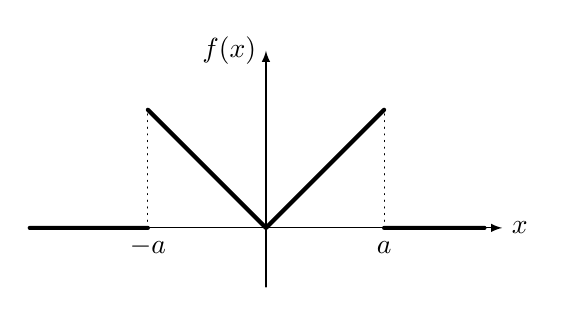
\begin{tikzpicture}[x = 1cm,		y = 1cm,		line join = round,		line cap = round,		> = latex, scale = 1.5,		]\draw[->]	(-2,0) -- (2,0)	node[right]	{$x$};\draw[->]	(0,-.5) --  (0,1.5)	node[left]	{$f(x)$};\draw[line width=1.5pt]		(-1,1) -- (0,0) --  (1,1)				(-2,0) -- (-1,0)				(1,0) -- (1.85,0);\draw[dotted]		(-1,0) node[below] {$-a$} -- (-1,1);\draw[dotted]		(1,0)  node[below] {$\vphantom{-}a$} -- (1,1);\end{tikzpicture}\end{figure}
 
\end{zkrPlain}

\vfil

\begin{zkrPlain}{25}\noindent 
	Отклонение количества изюма в кексах от среднего больше $15$ изюмин на кекс встречается в $68{,}27\%$ кексов. Кроме этого, замечено, что в $25{,}25\%$ случаев число изюминок в кексе меньше $70$. Найдите: \par \smallskip {\small \par \zz вероятность того, что изюминок в купленном кексе окажется от $90$ до $100$;\par \zz $4{,}78\%$-ную точку числа изюмин.}
 
\end{zkrPlain}

\vfil

\begin{zkrPlain}{25}\noindent 
	Вероятность сдачи в срок всех экзаменов студентом университета равна $ 0{,}08 $. Оцените вероятность того, что среди $ 720 $ студентов число сдавших в срок все экзамены отличается от своего математического ожидания не более чем на $ 20 $. 
 
\end{zkrPlain}

\newpage\setcounter{zad}{0}\setcounter{footnote}{0}



\begin{zkrPlain}{25}\noindent 
	Игральная кость подбрасывается до выпадения шестерки, но не более пяти раз. Случайная величина $X$ --- количество подбрасываний.  Найдите для этой случайной величины: \par \smallskip\small{ \par \zz ряд распределения (и постройте полигон); \par \zz функцию распределения (и постройте ее график); \par \zz математическое ожидание; \par \zz дисперсию и среднее квадратическое отклонение.\par \par}
 
\end{zkrPlain}

\vfil

\begin{zkrPlain}{25}\noindent 
	Найдите математическое ожидание, дисперсию и вероятность $P(X>a/2)$ непрерывной случайной величины с плотностью вероятностей $f(x)$, заданной графически\footnote{график может быть составлен лишь из участков прямых и парабол.}.\\ \begin{figure}[h!]\centering\small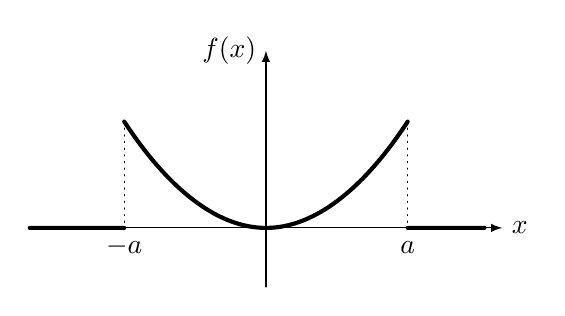
\begin{tikzpicture}[x = 1cm,		y = 1cm,		line join = round,		line cap = round,		> = latex, scale = 1.5,		]\draw[->]	(-2,0) -- (2,0)	node[right]	{$x$};\draw[->]	(0,-.5) --  (0,1.5)	node[left]	{$f(x)$};\draw[line width=1.5pt]		(0,0) parabola (1.2,.9);\draw[line width=1.5pt]		(0,0) parabola (-1.2,.9)				(-2,0) -- (-1.2,0)				(1.2,0) -- (1.85,0);\draw[dotted]	(-1.2,.9) -- (-1.2,0) node[below]	{$-a$};\draw[dotted]	(1.2,.9) -- (1.2,0) node[below]	{$\vphantom{-}a$};\end{tikzpicture}\end{figure}
 
\end{zkrPlain}

\vfil

\begin{zkrPlain}{25}\noindent 
	Средняя высота секвойи вечнозеленой  — порядка {$90$~м}. Примерно $1{,}31\%$ этих деревьев достигают в высоту $110$~м и более. Будем считать, что высота секвойи — нормально распределенная случайная величина. Найдите: \par \smallskip {\small \par \zz вероятность обнаружить секвойю высотой от $95$ до $105$ м;\par \zz вероятность того, что отклонение высоты случайной секвойи от средней составит не более десяти метров (по абсолютной величине).}
 
\end{zkrPlain}

\vfil

\begin{zkrPlain}{25}\noindent 
	Среднее значение длины детали $ 294 $ см, а дисперсия --- $ 276 $. Оцените вероятность того, что случайно взятая деталь окажется по длине не менее $ 243 $ и не более $ 345 $ см.
 
\end{zkrPlain}

\newpage\setcounter{zad}{0}\setcounter{footnote}{0}



\begin{zkrPlain}{25}\noindent 
	В ящике находятся 10 деталей, среди которых 5 бракованные. Наудачу из этих деталей вынимаются 4. Случайная величина $X$ --- количество бракованных деталей в выборке.  Найдите для этой случайной величины: \par \smallskip\small{ \par \zz ряд распределения (и постройте полигон); \par \zz функцию распределения (и постройте ее график); \par \zz математическое ожидание; \par \zz дисперсию и среднее квадратическое отклонение.\par \par}
 
\end{zkrPlain}

\vfil

\begin{zkrPlain}{25}\noindent 
	Найдите математическое ожидание, дисперсию и вероятность $P(X>a/2)$ непрерывной случайной величины с плотностью вероятностей $f(x)$, заданной графически\footnote{график может быть составлен лишь из участков прямых и парабол.}.\\ \begin{figure}[h!]\centering\small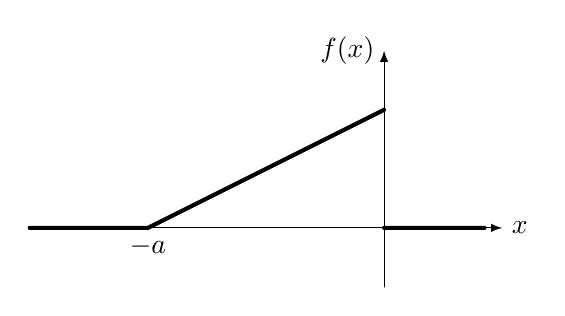
\begin{tikzpicture}[x = 1cm,		y = 1cm,		line join = round,		line cap = round,		> = latex, scale = 1.5,		]\draw[->]	(-3,0) -- (1,0)	node[right]	{$x$};\draw[->]	(0,-.5) --  (0,1.5)	node[left]	{$f(x)$};\draw[line width=1.5pt]		(-2,0) -- (0,1)				(-3,0) -- (-2,0)				(0,0) -- (.85,0);\draw[dotted]		(-2,0) node[below] {$-a$} -- (-2,0);\end{tikzpicture}\end{figure}
 
\end{zkrPlain}

\vfil

\begin{zkrPlain}{25}\noindent 
	Средний вес расфасованных пакетов со стиральным порошком $930$ г, но, как правило, около $6{,}68\%$ пакетов тяжелее $960$ г. Считаем, что вес пакетов распределен нормально. Найдите: \par \smallskip {\small \par \zz долю пакетов, имеющих вес до $900$ г.\par \zz Требуется, чтобы не более $4\%$ пакетов содержали меньше $900$ г порошка. На какой средний вес пакетов нужно переналадить фасовочный автомат для выполнения этого задания?}
 
\end{zkrPlain}

\vfil

\begin{zkrPlain}{25}\noindent 
	В течение времени $t$ экслуатируются $ 4500 $ приборов. Каждый прибор имеет надежность $ 0{,}6 $ и выходит из строя независимо от других. Оцените вероятность того, что в течение указанного времени выйдут из строя от $ 2585 $ до $ 2815 $ приборов.
 
\end{zkrPlain}

\newpage\setcounter{zad}{0}\setcounter{footnote}{0}



\begin{zkrPlain}{25}\noindent 
	Сотрудник лаборатории проводит пять независимых опытов. Вероятность успешного опыта равна $0{,}8$ и не зависит от успешности предыдущих опытов. Случайная величина $X$ --- число неудачных опытов.  Найдите для этой случайной величины: \par \smallskip\small{ \par \zz ряд распределения (и постройте полигон); \par \zz функцию распределения (и постройте ее график); \par \zz математическое ожидание; \par \zz дисперсию и среднее квадратическое отклонение.\par \par}
 
\end{zkrPlain}

\vfil

\begin{zkrPlain}{25}\noindent 
	Найдите математическое ожидание, дисперсию и вероятность $P(X>a/2)$ непрерывной случайной величины с плотностью вероятностей $f(x)$, заданной графически\footnote{график может быть составлен лишь из участков прямых и парабол.}.\\ \begin{figure}[h!]\centering\small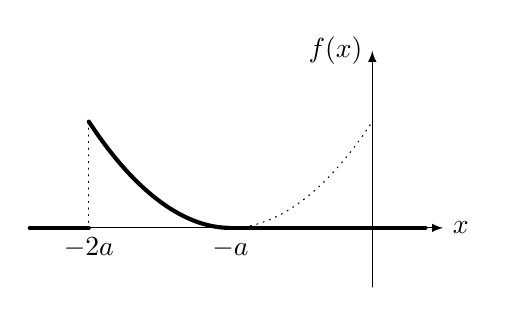
\begin{tikzpicture}[x = 1cm,		y = 1cm,		line join = round,		line cap = round,		> = latex, scale = 1.5,		]\draw[->]	(-.5,0) -- (3,0)	node[right]	{$x$};\draw[->]	(2.4,-.5) --  (2.4,1.5)	node[left]	{$f(x)$};\draw[line width=1.5pt]	(-.5,0) -- (0,0);\draw[line width=1.5pt]	(1.2,0) -- (2.85,0);\draw[dotted]		(1.2,0) parabola (2.4,.9);\draw[line width=1.5pt]		(1.2,0) node[below] {$-a$} parabola (0,.9);\draw[dotted]	(0,.9) -- (0,0) node[below] {$-2a$};\end{tikzpicture}\end{figure}
 
\end{zkrPlain}

\vfil

\begin{zkrPlain}{25}\noindent 
	Считаем, что рост императорского пингвина распределен нормально со средним квадратическим отклонением в три сантиметра. Известно, что $15{,}87\%$ императорских пингвинов имеют рост ниже $112$ см. Найдите: \par \smallskip {\small \par \zz долю императорских пингвинов с ростом от $116$ до $122$ см.;\par \zz с надежностью $0{,}9$ определить максимальное отклонение роста пингвина от его среднего значения.}
 
\end{zkrPlain}

\vfil

\begin{zkrPlain}{25}\noindent 
	В среднем $ 7 \% $ работоспособного населения некоторого региона --- безработные. Оцените вероятность того, что уровень безработицы среди обследованных $ 6900 $ работоспособных жителей города будет в пределах от $ 7 \% $ до $ 7 \% $.
 
\end{zkrPlain}

\newpage\setcounter{zad}{0}\setcounter{footnote}{0}



\begin{zkrPlain}{25}\noindent 
	Экзаменатор задает студенту вопросы до тех пор, пока не получит неверный ответ, но не более 3 вопросов. Вероятность того, что студент верно ответит на первый вопрос, равна $1/8$ и с каждым последующим вопросом увеличивается на $1/8$. Случайная величина $X$ --- число вопросов, заданных студенту.  Найдите для этой случайной величины: \par \smallskip\small{ \par \zz ряд распределения (и постройте полигон); \par \zz функцию распределения (и постройте ее график); \par \zz математическое ожидание; \par \zz дисперсию и среднее квадратическое отклонение.\par \par}
 
\end{zkrPlain}

\vfil

\begin{zkrPlain}{25}\noindent 
	Найдите математическое ожидание, дисперсию и вероятность $P(X>a/2)$ непрерывной случайной величины с плотностью вероятностей $f(x)$, заданной графически\footnote{график может быть составлен лишь из участков прямых и парабол.}.\\ \begin{figure}[h!]\centering\small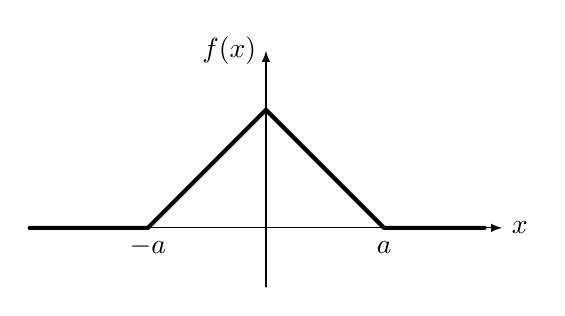
\begin{tikzpicture}[x = 1cm,		y = 1cm,		line join = round,		line cap = round,		> = latex, scale = 1.5,		]\draw[->]	(-2,0) -- (2,0)	node[right]	{$x$};\draw[->]	(0,-.5) --  (0,1.5)	node[left]	{$f(x)$};\draw[line width=1.5pt]		(-1,0) -- (0,1) --  (1,0)				(-2,0) -- (-1,0)				(1,0) -- (1.85,0);\draw[dotted]		(-1,0) node[below] {$-a$} -- (-1,0);\draw[dotted]		(1,0)  node[below] {$\vphantom{-}a$} -- (1,0);\end{tikzpicture}\end{figure}
 
\end{zkrPlain}

\vfil

\begin{zkrPlain}{25}\noindent 
	Сопротивление партии резисторов распределено по нормальному закону с номинальным средним значением $10$ кОм. Известно, что $84{,}13\%$ резисторов имеют сопротивление меньше $13$ кОм. Найдите: \par \smallskip {\small \par \zz вероятность того, что сопротивление выбранного наудачу резистора окажется в пределах от $9$ кОм до $11$ кОм;\par \zz с надежностью $90\%$ определить максимальное отклонение сопротивления от номинального среднего.}
 
\end{zkrPlain}

\vfil

\begin{zkrPlain}{25}\noindent 
	Вероятность того, что акции, переданные на депозит, будут востребованы, равна $ 0{,}08 $. Оцените вероятность того, что среди $ 710 $ клиентов от $ 37 $ до $ 77 $ востребуют свои акции.
 
\end{zkrPlain}

\newpage\setcounter{zad}{0}\setcounter{footnote}{0}



\begin{zkrPlain}{25}\noindent 
	На экзамен пришли пять студентов, уровень подготовки которых примерно одинаков. Вероятность того, что каждый студент завалит экзамен, равна $2/3$ и не зависит от результатов сдачи остальных. Случайная величина $X$ --- число студентов, заваливших экзамен.  Найдите для этой случайной величины: \par \smallskip\small{ \par \zz ряд распределения (и постройте полигон); \par \zz функцию распределения (и постройте ее график); \par \zz математическое ожидание; \par \zz дисперсию и среднее квадратическое отклонение.\par \par}
 
\end{zkrPlain}

\vfil

\begin{zkrPlain}{25}\noindent 
	Найдите математическое ожидание, дисперсию и вероятность $P(X>a/2)$ непрерывной случайной величины с плотностью вероятностей $f(x)$, заданной графически\footnote{график может быть составлен лишь из участков прямых и парабол.}.\\ \begin{figure}[h!]\centering\small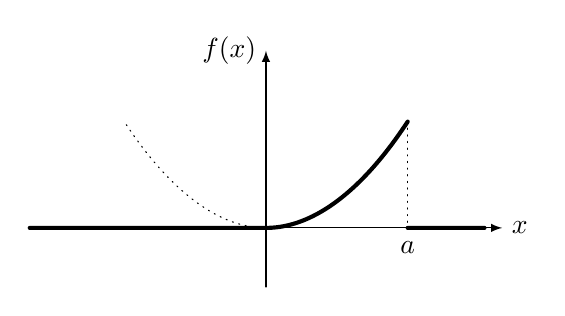
\begin{tikzpicture}[x = 1cm,		y = 1cm,		line join = round,		line cap = round,		> = latex, scale = 1.5,				]\draw[->]	(-2,0) -- (2,0)	node[right]	{$x$};\draw[->]	(0,-.5) --  (0,1.5)	node[left]	{$f(x)$};\draw[line width=1.5pt]	(0,0) parabola (1.2,.9)			(-2,0) -- (0,0)			(1.2,0) -- (1.85,0);\draw[dotted]	(0,0) parabola (-1.2,.9);\draw[dotted]	(1.2,.9) -- (1.2,0)	node[below]{$\vphantom{-}a$};\end{tikzpicture}\end{figure}
 
\end{zkrPlain}

\vfil

\begin{zkrPlain}{25}\noindent 
	По статистике ЕГЭ-2012 (русский язык), $7{,}66\%$ выпускников набрали менее $40$ баллов. Известно также, что $23{,}75\%$ выпускников получили более $70$ баллов. Считаем распределение баллов нормальным. Найдите: \par \smallskip {\small \par \zz средний балл по русскому языку;\par \zz долю отличников, получивших более $90$ баллов.}
 
\end{zkrPlain}

\vfil

\begin{zkrPlain}{25}\noindent 
	Среднее значение длины детали $ 41 $ см, а дисперсия --- $ 38 $. Оцените вероятность того, что случайно взятая деталь окажется по длине не менее $ 26 $ и не более $ 56 $ см.
 
\end{zkrPlain}

\newpage\setcounter{zad}{0}\setcounter{footnote}{0}



\begin{zkrPlain}{25}\noindent 
	В контрольной работе шесть задач. Вероятность правильного решения студентом каждой задачи равна $0{,}4$ и не зависит от правильности решения остальных. Случайная величина $X$ --- количество правильно решенных задач.  Найдите для этой случайной величины: \par \smallskip\small{ \par \zz ряд распределения (и постройте полигон); \par \zz функцию распределения (и постройте ее график); \par \zz математическое ожидание; \par \zz дисперсию и среднее квадратическое отклонение.\par \par}
 
\end{zkrPlain}

\vfil

\begin{zkrPlain}{25}\noindent 
	Найдите математическое ожидание, дисперсию и вероятность $P(X>a/2)$ непрерывной случайной величины с плотностью вероятностей $f(x)$, заданной графически\footnote{график может быть составлен лишь из участков прямых и парабол.}.\\ \begin{figure}[h!]\centering\small\begin{tikzpicture}[x = 1cm,		y = 1cm,		line join = round,		line cap = round,		> = latex, scale = 1.5,		]\draw[->]	(-.5,0) -- (3,0)	node[right]	{$x$};\draw[->]	(0,-.5) --  (0,1.5)	node[left]	{$f(x)$};\draw[line width=1.5pt]	(-.5,0) -- (0,0);\draw[line width=1.5pt]	(1.2,0) -- (2.85,0);\draw[dotted]		(1.2,0) parabola (2.4,.9);\draw[line width=1.5pt]		(1.2,0) parabola (0,.9);\draw[dotted]	(1.2,0) -- (1.2,0) node[below]	{$\vphantom{-}a$};\end{tikzpicture}\end{figure}
 
\end{zkrPlain}

\vfil

\begin{zkrPlain}{25}\noindent 
	Словарный запас английского языка у изучающих его — случайная величина, распределенная нормально. Известно, что в среднем этот запас составляет 8000 слов. Кроме этого, имеются данные, согласно которым $30{,}85\%$ изучающих имеют словарный запас менее $6000$ слов. Найдите: \par \smallskip {\small \par \zz долю изучающих английский со словарным запасом более $15000$ слов;\par \zz нижний квартиль ($x_{0{,}25}$)указанной случайной величины.}
 
\end{zkrPlain}

\vfil

\begin{zkrPlain}{25}\noindent 
	Вероятность сдачи в срок всех экзаменов студентом университета равна $ 0{,}07 $. Оцените вероятность того, что среди $ 3600 $ студентов число сдавших в срок все экзамены отличается от своего математического ожидания не более чем на $ 28 $. 
 
\end{zkrPlain}

\newpage\setcounter{zad}{0}\setcounter{footnote}{0}



\begin{zkrPlain}{25}\noindent 
	Противоположные грани кубика окрашены в красный, зеленый и синий цвета. Кубик подбрасывается 6 раз. Случайная величина $X$ --- количество подбрасываний, в результате которых сверху окажется грань, окрашенная в зеленый цвет.  Найдите для этой случайной величины: \par \smallskip\small{ \par \zz ряд распределения (и постройте полигон); \par \zz функцию распределения (и постройте ее график); \par \zz математическое ожидание; \par \zz дисперсию и среднее квадратическое отклонение.\par \par}
 
\end{zkrPlain}

\vfil

\begin{zkrPlain}{25}\noindent 
	Найдите математическое ожидание, дисперсию и вероятность $P(X>a/2)$ непрерывной случайной величины с плотностью вероятностей $f(x)$, заданной графически\footnote{график может быть составлен лишь из участков прямых и парабол.}.\\ \begin{figure}[h!]\centering\small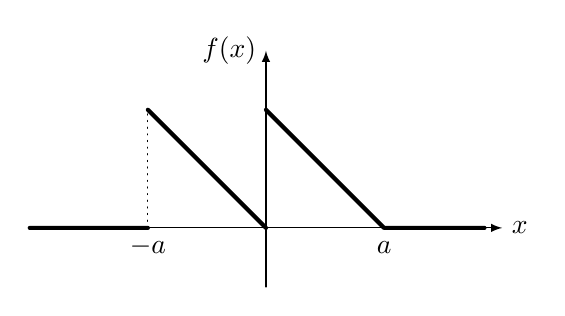
\begin{tikzpicture}[x = 1cm,		y = 1cm,		line join = round,		line cap = round,		> = latex, scale = 1.5,		]\draw[->]	(-2,0) -- (2,0)	node[right]	{$x$};\draw[->]	(0,-.5) --  (0,1.5)	node[left]	{$f(x)$};\draw[line width=1.5pt]		(-1,1) -- (0,0);\draw[line width=1.5pt]		(0,1) --  (1,0)				(-2,0) -- (-1,0)				(1,0) -- (1.85,0);\draw[dotted]		(-1,0) node[below] {$-a$} -- (-1,1);\draw[dotted]		(1,0)  node[below] {$\vphantom{-}a$} -- (1,0);\end{tikzpicture}\end{figure}
 
\end{zkrPlain}

\vfil

\begin{zkrPlain}{25}\noindent 
	Прочность пряжи приблизительно следует нормальному закону распределения. Средняя прочность пряжи — $245$ сн\footnote{1 сн (стен [тэ]) = 1000 ньютонов}. $1{,}22\%$ пряжи имеет прочность менее $200$ сн. Найдите: \par \smallskip {\small \par \zz вероятность того, что прочность окажется в интервале от $220$ сн до $270$ сн.\par \zz оценить наиболее вероятные границы прочности с помощью правила трех сигм.}
 
\end{zkrPlain}

\vfil

\begin{zkrPlain}{25}\noindent 
	Электростанция обслуживает сеть на $ 470 $ электроламп, вероятность включения которых утром равна $ 0{,}8 $. Оцените вероятность того, что число ламп, включенных в сеть сегодня утром, отличается от своего математического ожидания более чем на $ 22 $ (по абсолютной величине). 
 
\end{zkrPlain}

\newpage\setcounter{zad}{0}\setcounter{footnote}{0}



\begin{zkrPlain}{25}\noindent 
	Всхожесть семян данного сорта растений равна $45\%$. Посеяно пять семян. Случайная величина $X$ --- количество невзошедших семян из посеянных. Найдите для этой случайной величины: \par \smallskip\small{ \par \zz ряд распределения (и постройте полигон); \par \zz функцию распределения (и постройте ее график); \par \zz математическое ожидание; \par \zz дисперсию и среднее квадратическое отклонение.\par \par}
 
\end{zkrPlain}

\vfil

\begin{zkrPlain}{25}\noindent 
	Найдите математическое ожидание, дисперсию и вероятность $P(X>a/2)$ непрерывной случайной величины с плотностью вероятностей $f(x)$, заданной графически\footnote{график может быть составлен лишь из участков прямых и парабол.}.\\ \begin{figure}[h!]\centering\small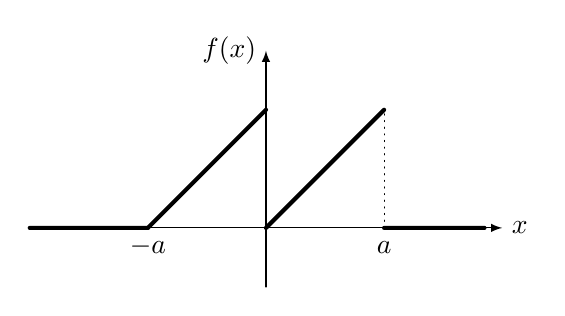
\begin{tikzpicture}[x = 1cm,		y = 1cm,		line join = round,		line cap = round,		> = latex, scale = 1.5,		]\draw[->]	(-2,0) -- (2,0)	node[right]	{$x$};\draw[->]	(0,-.5) --  (0,1.5)	node[left]	{$f(x)$};\draw[line width=1.5pt]		(-1,0) -- (0,1);\draw[line width=1.5pt]		(0,0)  --  (1,1)				(-2,0) -- (-1,0)				(1,0) -- (1.85,0);\draw[dotted]		(-1,0) node[below] {$-a$} -- (-1,0);\draw[dotted]		(1,0)  node[below] {$\vphantom{-}a$} -- (1,1);\end{tikzpicture}\end{figure}
 
\end{zkrPlain}

\vfil

\begin{zkrPlain}{25}\noindent 
	Максимальная урожайность большей части современных сортов картофеля — нормально распределенная случайная величина, принимающая $99{,}73\%$ своих значений в интервале $420-780$ ц/га. Найдите: \par \smallskip {\small \par \zz вероятность того, что урожайность высаженного картофеля в данном году составит от $650$ до $700$ ц/га;\par \zz $36{,}94\%$-ную точку указанной случайной величины.}
 
\end{zkrPlain}

\vfil

\begin{zkrPlain}{25}\noindent 
	В течение времени $t$ экслуатируются $ 5400 $ приборов. Каждый прибор имеет надежность $ 0{,}6 $ и выходит из строя независимо от других. Оцените вероятность того, что в течение указанного времени выйдут из строя от $ 3177 $ до $ 3303 $ приборов.
 
\end{zkrPlain}

\newpage\setcounter{zad}{0}\setcounter{footnote}{0}



\begin{zkrPlain}{25}\noindent 
	Среди 15 монет 5 --- фальшивые. Наудачу вынимают пять монет. Случайная величина $X$ --- количество фальшивых монет в выборке.  Найдите для этой случайной величины: \par \smallskip\small{ \par \zz ряд распределения (и постройте полигон); \par \zz функцию распределения (и постройте ее график); \par \zz математическое ожидание; \par \zz дисперсию и среднее квадратическое отклонение.\par \par}
 
\end{zkrPlain}

\vfil

\begin{zkrPlain}{25}\noindent 
	Найдите математическое ожидание, дисперсию и вероятность $P(X>a/2)$ непрерывной случайной величины с плотностью вероятностей $f(x)$, заданной графически\footnote{график может быть составлен лишь из участков прямых и парабол.}.\\ \begin{figure}[h!]\centering\small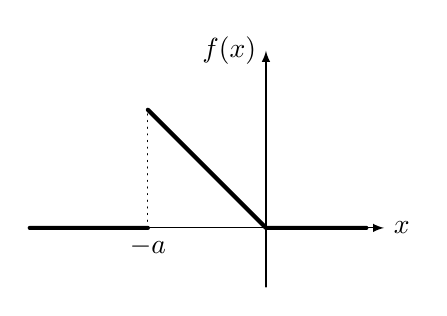
\begin{tikzpicture}[x = 1cm,		y = 1cm,		line join = round,		line cap = round,		> = latex, scale = 1.5,		]\draw[->]	(-2,0) -- (1,0)	node[right]	{$x$};\draw[->]	(0,-.5) --  (0,1.5)	node[left]	{$f(x)$};\draw[line width=1.5pt]		(-1,1) -- (0,0)				(-2,0) -- (-1,0)				(0,0) -- (.85,0);\draw[dotted]		(-1,0) node[below] {$-a$} -- (-1,1);\end{tikzpicture}\end{figure}
 
\end{zkrPlain}

\vfil

\begin{zkrPlain}{25}\noindent 
	Длина переднего рога у африканского белого носорога распределена по нормальному закону с параметром $\sigma = 5$ (см). Всего лишь $2{,}28\%$ белых носорогов имеют рог длиной более $100$ см. Найдите: \par \smallskip {\small \par \zz долю носорогов с рогом длиной от $85$ см до $95$ см;\par \zz квантиль уровня $0{,}3$.}
 
\end{zkrPlain}

\vfil

\begin{zkrPlain}{25}\noindent 
	Электростанция обслуживает сеть на $ 2400 $ электроламп, вероятность включения которых утром равна $ 0{,}7 $. Оцените вероятность того, что число ламп, включенных в сеть сегодня утром, отличается от своего математического ожидания более чем на $ 89 $ (по абсолютной величине). 
 
\end{zkrPlain}

\newpage\setcounter{zad}{0}\setcounter{footnote}{0}



\begin{zkrPlain}{25}\noindent 
	В корзине 5 синих и 7 красных мячей. Наудачу вынимают четыре мяча. Случайная величина $X$ --- количество красных мячей в выборке.  Найдите для этой случайной величины: \par \smallskip\small{ \par \zz ряд распределения (и постройте полигон); \par \zz функцию распределения (и постройте ее график); \par \zz математическое ожидание; \par \zz дисперсию и среднее квадратическое отклонение.\par \par}
 
\end{zkrPlain}

\vfil

\begin{zkrPlain}{25}\noindent 
	Найдите математическое ожидание, дисперсию и вероятность $P(X>a/2)$ непрерывной случайной величины с плотностью вероятностей $f(x)$, заданной графически\footnote{график может быть составлен лишь из участков прямых и парабол.}.\\ \begin{figure}[h!]\centering\small\begin{tikzpicture}[x = 1cm,		y = 1cm,		line join = round,		line cap = round,		> = latex, scale = 1.5,		]\draw[->]	(-2,0) -- (2,0)	node[right]	{$x$};\draw[->]	(0,-.5) --  (0,1.5)	node[left]	{$f(x)$};\draw[line width=1.5pt]	(0,1) parabola (1.5,0) node[below] {$\vphantom{-}a$}			(-2,0) -- (0,0)			(1.5,0) -- (1.85,0);\draw[dotted] (0,1) parabola (-1.5,0);\end{tikzpicture}\end{figure}
 
\end{zkrPlain}

\vfil

\begin{zkrPlain}{25}\noindent 
	Вес рыб, обитающих в водоеме, подчиняется нормальному закону с параметром $a = 375$ г. Вероятность того, что вес пойманной рыбы меньше $400$ г, равна $0{,}8413$. Найдите: \par \smallskip {\small \par \zz вероятность того, что вес выловленной наудачу рыбы попадет в промежуток от $300$ г до $425$ г;\par \zz квантиль уровня $0{,}7$.}
 
\end{zkrPlain}

\vfil

\begin{zkrPlain}{25}\noindent 
	Вероятность того, что акции, переданные на депозит, будут востребованы, равна $ 0{,}06 $. Оцените вероятность того, что среди $ 770 $ клиентов от $ 31 $ до $ 61 $ востребуют свои акции.
 
\end{zkrPlain}

\newpage\setcounter{zad}{0}\setcounter{footnote}{0}



\begin{zkrPlain}{25}\noindent 
	Секретариат фирмы оборудован четырьмя независимо работающими компьютерами. Вероятность отказа каждого из них в течение рабочего дня равна $20\%$. Случайная величина $X$ --- количество отказавших в течение рабочего дня компьютеров.  Найдите для этой случайной величины: \par \smallskip\small{ \par \zz ряд распределения (и постройте полигон); \par \zz функцию распределения (и постройте ее график); \par \zz математическое ожидание; \par \zz дисперсию и среднее квадратическое отклонение.\par \par}
 
\end{zkrPlain}

\vfil

\begin{zkrPlain}{25}\noindent 
	Найдите математическое ожидание, дисперсию и вероятность $P(X>a/2)$ непрерывной случайной величины с плотностью вероятностей $f(x)$, заданной графически\footnote{график может быть составлен лишь из участков прямых и парабол.}.\\ \begin{figure}[h!]\centering\small\begin{tikzpicture}[x = 1cm,		y = 1cm,		line join = round,		line cap = round,		> = latex, scale = 1.5,		]\draw[->]	(-1,0) -- (3,0)	node[right]	{$x$};\draw[->]	(0,-.5) --  (0,1.5)	node[left]	{$f(x)$};\draw[line width=1.5pt]		 (0,1) --  (2,0)				(-1,0) -- (0,0)				(2,0) -- (2.85,0);\draw[dotted]		(2,0)  node[below] {$\vphantom{-}a$} -- (2,0);\end{tikzpicture}\end{figure}
 
\end{zkrPlain}

\vfil

\begin{zkrPlain}{25}\noindent 
	Вес товаров, помещаемых в контейнер определенного размера, — нормально распределенная случайная величина. Известно, что $34{,}46\%$ контейнеров имеют чистый вес меньше $8$ тонн и $21{,}19\%$ имеют вес больше, чем $14$ тонн. Найдите: \par \smallskip {\small \par \zz средний вес одного контейнера; \par \zz с надежностью $0{,}9$ максимальное отклонение веса контейнера от среднего значения. }
 
\end{zkrPlain}

\vfil

\begin{zkrPlain}{25}\noindent 
	В среднем $ 6 \% $ работоспособного населения некоторого региона --- безработные. Оцените вероятность того, что уровень безработицы среди обследованных $ 2300 $ работоспособных жителей города будет в пределах от $ 5 \% $ до $ 7 \% $.
 
\end{zkrPlain}

\newpage\setcounter{zad}{0}\setcounter{footnote}{0}



\begin{zkrPlain}{25}\noindent 
	В ящике находятся 5 белых и 5 черных шаров. Случайным образом последовательно вынимаются шары до появления белого шара. Шары не возвращаются в ящик. Случайная величина $X$ --- количество вынутых шаров.  Найдите для этой случайной величины: \par \smallskip\small{ \par \zz ряд распределения (и постройте полигон); \par \zz функцию распределения (и постройте ее график); \par \zz математическое ожидание; \par \zz дисперсию и среднее квадратическое отклонение.\par \par}
 
\end{zkrPlain}

\vfil

\begin{zkrPlain}{25}\noindent 
	Найдите математическое ожидание, дисперсию и вероятность $P(X>a/2)$ непрерывной случайной величины с плотностью вероятностей $f(x)$, заданной графически\footnote{график может быть составлен лишь из участков прямых и парабол.}.\\ \begin{figure}[h!]\centering\small\begin{tikzpicture}[x = 1cm,		y = 1cm,		line join = round,		line cap = round,		> = latex, scale = 1.5,		]\draw[->]	(-2.5,0) -- (1.5,0)	node[right]	{$x$};\draw[->]	(0,-.5) --  (0,1.5)	node[left]	{$f(x)$};\draw[line width=1.5pt]		(-1.2,0) node[below] {$-a$} parabola (0,.9);\draw[line width=1.5pt]		(-2.5,0) -- (-1.2,0)				(0,0) -- (1.35,0);\draw[dotted]	(-1.2,0) parabola (-2.4,.9);\end{tikzpicture}\end{figure}
 
\end{zkrPlain}

\vfil

\begin{zkrPlain}{25}\noindent 
	Средний рост представителя пигмейских народов гиелли и эфе равен $147$ см. Известно также, что «высоких» людей (выше $1{,}5$ м) среди этих народов — лишь $0{,}13\%$. Учесть, что рост человека (хотя бы и пигмея) распределен нормально. Найдите: \par \smallskip {\small \par \zz долю пигмеев, имеющих рост от $146$ до $148$ см ;\par \zz квантиль уровня $0{,}0227$ описанной случайной величины.}
 
\end{zkrPlain}

\vfil

\begin{zkrPlain}{25}\noindent 
	Вероятность сдачи в срок всех экзаменов студентом университета равна $ 0{,}05 $. Оцените вероятность того, что среди $ 5400 $ студентов число сдавших в срок все экзамены отличается от своего математического ожидания не более чем на $ 29 $. 
 
\end{zkrPlain}

\newpage\setcounter{zad}{0}\setcounter{footnote}{0}



\begin{zkrPlain}{25}\noindent 
	Среди партии шарфов, поступивших в магазин, $70 \%$ составляют однотонные шарфы, а остальные --- пестрые. Покупатель из этих шарфов случайным образом выбирает три. Случайная величина $X$ --- количество пестрых шарфов в выборке.  Найдите для этой случайной величины: \par \smallskip\small{ \par \zz ряд распределения (и постройте полигон); \par \zz функцию распределения (и постройте ее график); \par \zz математическое ожидание; \par \zz дисперсию и среднее квадратическое отклонение.\par \par}
 
\end{zkrPlain}

\vfil

\begin{zkrPlain}{25}\noindent 
	Найдите математическое ожидание, дисперсию и вероятность $P(X>a/2)$ непрерывной случайной величины с плотностью вероятностей $f(x)$, заданной графически\footnote{график может быть составлен лишь из участков прямых и парабол.}.\\ \begin{figure}[h!]\centering\small\begin{tikzpicture}[x = 1cm,		y = 1cm,		line join = round,		line cap = round,		> = latex, scale = 1.5,		]\draw[->]	(-2,0) -- (2,0)	node[right]	{$x$};\draw[->]	(0,-.5) --  (0,1.5)	node[left]	{$f(x)$};\draw[line width=1.5pt]		(-1,1) --  (1,0)				(-2,0) -- (-1,0)				(1,0) -- (1.85,0);\draw[dotted]		(-1,0) node[below] {$-a$} -- (-1,1);\draw[dotted]		(1,0)  node[below] {$\vphantom{-}a$} -- (1,0);\end{tikzpicture}\end{figure}
 
\end{zkrPlain}

\vfil

\begin{zkrPlain}{25}\noindent 
	По статистике ЕГЭ-2012 по математике, $15{,}87\%$ выпускников набрали менее $30$ баллов. Среднее число набранных баллов — $45$. Будем считать число баллов распределенным нормально. Найдите: \par \smallskip {\small \par \zz долю выпускников, набравших более $90$ баллов;\par \zz квантиль уровня $0{,}9522$ числа набранных баллов.}
 
\end{zkrPlain}

\vfil

\begin{zkrPlain}{25}\noindent 
	Среднее значение длины детали $ 47 $ см, а дисперсия --- $ 44 $. Оцените вероятность того, что случайно взятая деталь окажется по длине не менее $ 24 $ и не более $ 70 $ см.
 
\end{zkrPlain}

\newpage\setcounter{zad}{0}\setcounter{footnote}{0}



\begin{zkrPlain}{25}\noindent 
	На маршруте работают три автобуса. Вероятность поломки каждого из них в течение рабочего дня равна $0{,}9$ и не зависит от состояния остальных. Случайная величина $X$ --- число неисправных в течение рабочего дня автобусов.  Найдите для этой случайной величины: \par \smallskip\small{ \par \zz ряд распределения (и постройте полигон); \par \zz функцию распределения (и постройте ее график); \par \zz математическое ожидание; \par \zz дисперсию и среднее квадратическое отклонение.\par \par}
 
\end{zkrPlain}

\vfil

\begin{zkrPlain}{25}\noindent 
	Найдите математическое ожидание, дисперсию и вероятность $P(X>a/2)$ непрерывной случайной величины с плотностью вероятностей $f(x)$, заданной графически\footnote{график может быть составлен лишь из участков прямых и парабол.}.\\ \begin{figure}[h!]\centering\small\begin{tikzpicture}[x = 1cm,		y = 1cm,		line join = round,		line cap = round,		> = latex, scale = 1.5,		]\draw[->]	(-.5,0) -- (3,0)	node[right]	{$x$};\draw[->]	(2.4,-.5) --  (2.4,1.5)	node[left]	{$f(x)$};\draw[line width=1.5pt]	(-.5,0) -- (0,0);\draw[line width=1.5pt]	(1.2,0) -- (2.85,0);\draw[dotted]		(1.2,0) parabola (2.4,.9);\draw[line width=1.5pt]		(1.2,0) node[below] {$-a$} parabola (0,.9);\draw[dotted]	(0,.9) -- (0,0) node[below] {$-2a$};\end{tikzpicture}\end{figure}
 
\end{zkrPlain}

\vfil

\begin{zkrPlain}{25}\noindent 
	Спортсмен бросает копье. Дальность полета — нормально распределенная величина со средним значением $70$ м. По статистике $2{,}28\%$ бросков, как правило, оказываются неудачными (дальность полета менее $60$ м).  Найдите: \par \smallskip {\small \par \zz  вероятность того, что копье упадет на расстоянии от $65$ м до $75$ м.\par \zz нижний квартиль распределения ($x_{0{,}25}$).}
 
\end{zkrPlain}

\vfil

\begin{zkrPlain}{25}\noindent 
	Среднее значение длины детали $ 17 $ см, а дисперсия --- $ 16 $. Оцените вероятность того, что случайно взятая деталь окажется по длине не менее $ 13 $ и не более $ 21 $ см.
 
\end{zkrPlain}

\newpage\setcounter{zad}{0}\setcounter{footnote}{0}



\begin{zkrPlain}{25}\noindent 
	Из букв слова СТАТИСТИКА случайным образом выбирают 4 буквы. Случайная величина $X$--- количество гласных букв в выборке. Найдите для этой случайной величины: \par \smallskip\small{ \par \zz ряд распределения (и постройте полигон); \par \zz функцию распределения (и постройте ее график); \par \zz математическое ожидание; \par \zz дисперсию и среднее квадратическое отклонение.\par \par}
 
\end{zkrPlain}

\vfil

\begin{zkrPlain}{25}\noindent 
	Найдите математическое ожидание, дисперсию и вероятность $P(X>a/2)$ непрерывной случайной величины с плотностью вероятностей $f(x)$, заданной графически\footnote{график может быть составлен лишь из участков прямых и парабол.}.\\ \begin{figure}[h!]\centering\small\begin{tikzpicture}[x = 1cm,		y = 1cm,		line join = round,		line cap = round,		> = latex, scale = 1.5,		]\draw[->]	(-2.5,0) -- (1.5,0)	node[right]	{$x$};\draw[->]	(0,-.5) --  (0,1.5)	node[left]	{$f(x)$};\draw[line width=1.5pt]		(-1.2,0) node[below] {$-a$} parabola (0,.9);\draw[line width=1.5pt]		(-2.5,0) -- (-1.2,0)				(0,0) -- (1.35,0);\draw[dotted]	(-1.2,0) parabola (-2.4,.9);\end{tikzpicture}\end{figure}
 
\end{zkrPlain}

\vfil

\begin{zkrPlain}{25}\noindent 
	Вес гигантского броненосца — нормально распределенная случайная величина. Известно, что $74{,}75\%$ этих животных в весе не превышают $27$ кг, а тяжелее $30$ кг — лишь $4{,}78\%$ броненосцев. Найдите: \par \smallskip {\small \par \zz вероятность случайно встретить в джунглях броненосца весом менее $22$ кг;\par \zz $9{,}12\%$-ную точку данной случайной величины.}
 
\end{zkrPlain}

\vfil

\begin{zkrPlain}{25}\noindent 
	В среднем $ 5 \% $ работоспособного населения некоторого региона --- безработные. Оцените вероятность того, что уровень безработицы среди обследованных $ 350 $ работоспособных жителей города будет в пределах от $ 4 \% $ до $ 7 \% $.
 
\end{zkrPlain}

\newpage\setcounter{zad}{0}\setcounter{footnote}{0}



\begin{zkrPlain}{25}\noindent 
	Экзаменатор задает студенту вопросы до тех пор, пока не получит верный ответ, но не более 3 вопросов. Вероятность того, что студент неверно ответит на первый вопрос, равна $6/7$ и с каждым последующим вопросом уменьшается на $1/7$. Случайная величина $X$ --- число вопросов, заданных студенту.  Найдите для этой случайной величины: \par \smallskip\small{ \par \zz ряд распределения (и постройте полигон); \par \zz функцию распределения (и постройте ее график); \par \zz математическое ожидание; \par \zz дисперсию и среднее квадратическое отклонение.\par \par}
 
\end{zkrPlain}

\vfil

\begin{zkrPlain}{25}\noindent 
	Найдите математическое ожидание, дисперсию и вероятность $P(X>a/2)$ непрерывной случайной величины с плотностью вероятностей $f(x)$, заданной графически\footnote{график может быть составлен лишь из участков прямых и парабол.}.\\ \begin{figure}[h!]\centering\small\begin{tikzpicture}[x = 1cm,		y = 1cm,		line join = round,		line cap = round,		> = latex, scale = 1.5,		]\draw[->]	(-2,0) -- (2,0)	node[right]	{$x$};\draw[->]	(0,-.5) --  (0,1.5)	node[left]	{$f(x)$};\draw[line width=1.5pt]		(-1,0) -- (1,1)				(-2,0) -- (-1,0)				(1,0) -- (1.85,0);\draw[dotted]		(-1,0) node[below] {$-a$} -- (-1,0);\draw[dotted]		(1,0)  node[below] {$\vphantom{-}a$} -- (1,1);\end{tikzpicture}\end{figure}
 
\end{zkrPlain}

\vfil

\begin{zkrPlain}{25}\noindent 
	Уровень воды в реке — случайная величина со средним значением $2{,}5$ м. Вероятность того, что в наудачу выбранный день уровень воды в реке окажется больше $3$ м, равна $0{,}62\%$. Найдите: \par \smallskip {\small \par \zz  вероятность того, что уровень воды в случайный день окажется в пределах от $240$ см до $270$ см;\par \zz $15\%$-ную точку этой случайной величины.}
 
\end{zkrPlain}

\vfil

\begin{zkrPlain}{25}\noindent 
	В течение времени $t$ экслуатируются $ 2700 $ приборов. Каждый прибор имеет надежность $ 0{,}7 $ и выходит из строя независимо от других. Оцените вероятность того, что в течение указанного времени выйдут из строя от $ 1821 $ до $ 1959 $ приборов.
 
\end{zkrPlain}

\newpage\setcounter{zad}{0}\setcounter{footnote}{0}



\begin{zkrPlain}{25}\noindent 
	В рекламных целях торговая фирма вкладывает в каждую десятую единицу товара денежный приз размером 100 рублей. Случайная величина $X$ --- размер выигрыша при трех сделанных покупках.  Найдите для этой случайной величины: \par \smallskip\small{ \par \zz ряд распределения (и постройте полигон); \par \zz функцию распределения (и постройте ее график); \par \zz математическое ожидание; \par \zz дисперсию и среднее квадратическое отклонение.\par \par}
 
\end{zkrPlain}

\vfil

\begin{zkrPlain}{25}\noindent 
	Найдите математическое ожидание, дисперсию и вероятность $P(X>a/2)$ непрерывной случайной величины с плотностью вероятностей $f(x)$, заданной графически\footnote{график может быть составлен лишь из участков прямых и парабол.}.\\ \begin{figure}[h!]\centering\small\begin{tikzpicture}[x = 1cm,		y = 1cm,		line join = round,		line cap = round,		> = latex, scale = 1.5,				]\draw[->]	(-2,0) -- (2,0)	node[right]	{$x$};\draw[->]	(0,-.5) --  (0,1.5)	node[left]	{$f(x)$};\draw[line width=1.5pt]	(0,0) parabola (1.2,.9)			(-2,0) -- (0,0)			(1.2,0) -- (1.85,0);\draw[dotted]	(0,0) parabola (-1.2,.9);\draw[dotted]	(1.2,.9) -- (1.2,0)	node[below]{$\vphantom{-}a$};\end{tikzpicture}\end{figure}
 
\end{zkrPlain}

\vfil

\begin{zkrPlain}{25}\noindent 
	Коробки с шоколадом упаковываются автоматически. Их средняя масса равна $1{,}2$ кг. Известно, что $9{,}68\%$ коробок имеют массу, меньшую $1{,}07$ кг. Предполагается, что масса коробки распределена нормально. Найдите: \par \smallskip {\small \par \zz процент коробок с массой, превышающей $1140$ г;\par \zz $30\%$-ную точку распределения.}
 
\end{zkrPlain}

\vfil

\begin{zkrPlain}{25}\noindent 
	Электростанция обслуживает сеть на $ 3500 $ электроламп, вероятность включения которых утром равна $ 0{,}5 $. Оцените вероятность того, что число ламп, включенных в сеть сегодня утром, отличается от своего математического ожидания более чем на $ 58 $ (по абсолютной величине). 
 
\end{zkrPlain}

\newpage\setcounter{zad}{0}\setcounter{footnote}{0}



\begin{zkrPlain}{25}\noindent 
	Стрелок ведет стрельбу по цели с вероятностью промаха при каждом выстреле $75\%$. За каждое попадание он получает 10 очков, а в случае промаха очков ему не начисляют. Случайная величина $X$ --- число очков, полученных стрелком за 6 выстрелов.  Найдите для этой случайной величины: \par \smallskip\small{ \par \zz ряд распределения (и постройте полигон); \par \zz функцию распределения (и постройте ее график); \par \zz математическое ожидание; \par \zz дисперсию и среднее квадратическое отклонение.\par \par}
 
\end{zkrPlain}

\vfil

\begin{zkrPlain}{25}\noindent 
	Найдите математическое ожидание, дисперсию и вероятность $P(X>a/2)$ непрерывной случайной величины с плотностью вероятностей $f(x)$, заданной графически\footnote{график может быть составлен лишь из участков прямых и парабол.}.\\ \begin{figure}[h!]\centering\small\begin{tikzpicture}[x = 1cm,		y = 1cm,		line join = round,		line cap = round,		> = latex, scale = 1.5,		]\draw[->]	(-3,0) -- (1,0)	node[right]	{$x$};\draw[->]	(0,-.5) --  (0,1.5)	node[left]	{$f(x)$};\draw[line width=1.5pt]		(-2,1) -- (0,0)				(-3,0) -- (-2,0)				(0,0) -- (.85,0);\draw[dotted]		(-2,0) node[below] {$-a$} -- (-2,1);\end{tikzpicture}\end{figure}
 
\end{zkrPlain}

\vfil

\begin{zkrPlain}{25}\noindent 
	Тесты IQ разрабатываются так, чтобы их результаты описывались нормальным распределением со средним значением $100$ и с таким разбросом, чтобы $25\%$ тестируемых имели IQ ниже $90$. Найдите: \par \smallskip {\small \par \zz вероятность случайному испытуемому получить по результатам теста IQ от $110$  до $120$;\par \zz с помощью правила трех сигм границы, в которых находится IQ большинства людей.}
 
\end{zkrPlain}

\vfil

\begin{zkrPlain}{25}\noindent 
	Вероятность сдачи в срок всех экзаменов студентом университета равна $ 0{,}05 $. Оцените вероятность того, что среди $ 740 $ студентов число сдавших в срок все экзамены отличается от своего математического ожидания не более чем на $ 14 $. 
 
\end{zkrPlain}

\newpage\setcounter{zad}{0}\setcounter{footnote}{0}



\begin{zkrPlain}{25}\noindent 
		Вероятность заболеть гриппом в период эпидемии составляет $1/2$. Рассматривается контрольная группа, состоящая из пяти человек. Случайная величина $X$ --- количество заболевших в период эпидемии человек данной группы.  Найдите для этой случайной величины: \par \smallskip\small{ \par \zz ряд распределения (и постройте полигон); \par \zz функцию распределения (и постройте ее график); \par \zz математическое ожидание; \par \zz дисперсию и среднее квадратическое отклонение.\par \par}
 
\end{zkrPlain}

\vfil

\begin{zkrPlain}{25}\noindent 
	Найдите математическое ожидание, дисперсию и вероятность $P(X>a/2)$ непрерывной случайной величины с плотностью вероятностей $f(x)$, заданной графически\footnote{график может быть составлен лишь из участков прямых и парабол.}.\\ \begin{figure}[h!]\centering\small\begin{tikzpicture}[x = 1cm,		y = 1cm,		line join = round,		line cap = round,		> = latex, scale = 1.5,		]\draw[->]	(-2,0) -- (1,0)	node[right]	{$x$};\draw[->]	(0,-.5) --  (0,1.5)	node[left]	{$f(x)$};\draw[line width=1.5pt]		(-1,1) -- (0,0)				(-2,0) -- (-1,0)				(0,0) -- (.85,0);\draw[dotted]		(-1,0) node[below] {$-a$} -- (-1,1);\end{tikzpicture}\end{figure}
 
\end{zkrPlain}

\vfil

\begin{zkrPlain}{25}\noindent 
	Изменение индекса ценной бумаги на фондовой бирже может быть смоделировано как нормально распределенная случайная величина с параметром $\sigma^2 = 0{,}01$. Известно также, что на следующих торгах с вероятностью $0{,}0228$ изменение индекса будет менее $0{,}8$. Найдите: \par \smallskip {\small \par \zz вероятность того, что на следующих торгах изменение индекса будет больше $1{,}2$.\par \zz нижний квартиль ($x_{0{,}25}$) этой случайной величины.}
 
\end{zkrPlain}

\vfil

\begin{zkrPlain}{25}\noindent 
	Вероятность того, что акции, переданные на депозит, будут востребованы, равна $ 0{,}07 $. Оцените вероятность того, что среди $ 430 $ клиентов от $ 15 $ до $ 45 $ востребуют свои акции.
 
\end{zkrPlain}

\newpage\setcounter{zad}{0}\setcounter{footnote}{0}

